\documentclass[
  draft=false,
  paper=a4,
  twoside=false,
  fontsize=11pt,
  headsepline,
  BCOR10mm,
  DIV11
]{scrbook}

\usepackage[T1]{fontenc}
\usepackage[utf8]{inputenc}
\usepackage[ngerman, english]{babel}
\usepackage{textcomp}
\usepackage{libertine}
\usepackage{pifont}
\usepackage{microtype}
\usepackage{textcomp}
\usepackage[german,refpage]{nomencl}
\usepackage{setspace}
\usepackage{makeidx}
\usepackage{listings}
\usepackage{natbib}
\usepackage[ngerman,colorlinks=true]{hyperref}
\usepackage{soul}
\usepackage{hawstyle}
\usepackage{epigraph}

% Custom packages 
\usepackage{scrhack}
\usepackage{graphicx}
\usepackage{algorithm,algpseudocode}
\usepackage{amsmath}
\usepackage{kbordermatrix} % http://www.hss.caltech.edu/~kcb/LaTeX.shtml

\colorlet{BackgroundColor}{gray!20}
\colorlet{KeywordColor}{blue}
\colorlet{CommentColor}{black!60}
\colorlet{HeadColor}{gray!60}
\colorlet{Color1}{blue!10}
\colorlet{Color2}{white}

\HAWifprinter{
  \colorlet{BackgroundColor}{gray!20}
  \colorlet{KeywordColor}{black}
  \colorlet{CommentColor}{gray}
  \colorlet{HeadColor}{gray!60}
  \colorlet{Color1}{gray!40}
  \colorlet{Color2}{white}
}{}

\lstset{
  numbers=left,
  numberstyle=\tiny,
  stepnumber=1,
  numbersep=5pt,
  basicstyle=\ttfamily\small,
  keywordstyle=\color{KeywordColor}\bfseries,
  identifierstyle=\color{black},
  commentstyle=\color{CommentColor},
  backgroundcolor=\color{BackgroundColor},
  captionpos=b,
  fontadjust=true
}

\lstset{escapeinside={(*@}{@*)}, % used to enter latex code inside listings
  morekeywords={uint32_t, int32_t}
}

\ifpdfoutput{
  \hypersetup{bookmarksopen=false,bookmarksnumbered,linktocpage}
}{}

\DeclareRobustCommand{\cxx}{C\raisebox{0.25ex}{{\scriptsize +\kern-0.25ex +}}}

\clubpenalty=10000
\widowpenalty=10000
\displaywidowpenalty=10000

\hyphenation{}

\typearea[current]{last}

\lstset{
  frame = single,
  basicstyle=\ttfamily\small,
  fontadjust=true
}

\setcounter{tocdepth}{3}
\setcounter{secnumdepth}{3}

\makeindex
\makenomenclature

\begin{document}
  \HAWThesisProperties{
    Author={Matthias Nitsche},
    Title={Continuous Clustering for a Daily News Summarization System},
    EnglishTitle={Continuous Clustering for a Daily News Summarization System},
    ThesisType={Bachelorarbeit},
    ExaminationType={Bachelorprüfung},
    DegreeProgramme={Bachelor of Science Angewandte Informatik},
    ThesisExperts={Prof. Dr. Michael Neitzke \and Prof. Dr. Olaf Zukunft},
    ReleaseDate={06. February 2016}
  }


  \frontmatter
    \maketitle
    \onehalfspacing

    \HAWAbstractPage
  {
    Clustering, Cluster Analyse, 
    Dokument Clustering, Vector Space Model,
    Partitionelles Clustering,
    Hierarchisches Clustering,
    Probabilistic Topic Modeling, 
    Text Zusammenfassung,
    Text Mining, Data Mining,
    Machinelles Lernen, Unüberwachtes Lernen, 
    Information Retrieval
  }
  { 
    Für eine Maschine ist es schwer, ohne die Supervision eines menschlichen Expertens text zu interpretieren. Techniken des Text Minings und clustern als Ansatz von unsupervisierten Lernen, um Text aus Zeitungen in Kategorien und zu Ereignissen in der realen Welt zu gruppieren, ist zentral in dieser Arbeit. Zusätzlich, wurde ein funktionierendes Datenverarbeitungssystem, zum herunterladen und verarbeiten von Zeitungsartikeln, entwickelt, um clustering Algorithmen eine Grundlage zu geben. In kurz, die präsentierten Selektionsstrategien und clustering Algorithmen haben eine ähnliche Wirkung.
  }
  { 
    Clustering, Cluster Analysis, 
    Document Clustering, Vector Space Model,
    Partitional Clustering,
    Hierarchical Clustering,
    Probabilistic Topic Modeling,
    Summarization,
    Text Mining, Data Mining,
    Machine Learning, Unsupervised Learning, 
    Information Retrieval
  }
  {
    Interpreting and summarizing textual content without the supervision of human experts is subject of this thesis. Using techniques of text mining and document clustering as an approach of unsupervised machine learning, grouping textual content of online newspaper articles, into coherent categories and real world events is subject of this thesis. Additionally, building a functioning data pipeline for scraping and preprocessing newspaper articles, feeding clustering algorithms, shows promising results. In short, the presented feature selection and clustering strategies yield similar effects.
  }




    \newpage

    \singlespacing
    \tableofcontents

    \newpage
    \listoftables
    \listoffigures
    %\lstlistoflistings


  \mainmatter
    \onehalfspacing
    \typeout{===== File: chapter 1}

    \chapter{Introduction}
      \label{chapter:introduction}
      \epigraph{\emph{
  ``Where there is matter, there is geometry.''
}}{ Johannes Kepler }

\paragraph{} Text mining and natural language processing have long been studied in the field of artificial intelligence. Within the last decade, models that are computationally expensive, were reopened for discussion. Machine learning aids in this task by approximating models for structured and unstructured data. Recognizing patterns, retrieving information or classifying content of interest for huge data sets, often scaled over thousands of machines. This process is called knowledge discovery. By continuously clustering daily news articles to summarize them, the task at hand is simple: Reducing noise which surrounds textual documents by presenting the useful fraction of information. The useful fraction of information can be anything from topic detection to summarization providing additional reasoning for humans. Mining documents, preprocessing them into suitable representations and grouping their form to detect underlying patterns that connect documents is the primary goal of this thesis.

\paragraph{} It goes without saying that newspaper articles are created by humans. While automation and easy retrieval can be of utmost importance, news are created by authors, journalists, generally professional writers. The main purpose of text mining is to scale suitable algorithms to data sets, that are too enormous to be comprehended by a single person. Without authors there is no text, therefore the highest good at hand are the documents by the authors.

\paragraph{} In the following we will examine the field of unsupervised learning with respect to clustering exemplified by a news clustering system. The objective is to build parts of an automatic summarization system that scrapes newspapers, preprocesses the content and groups them into clusters for summarization purposes.\\
We will soon see that assumptions from linear algebra and geometry will be of utmost importance to understand text representation. Essentially it is all about smart counting. This sentiment lines up with the quote by Johannes Keppler ``Where there is matter, there is geometry.''

\section{Machine Learning}
\label{sec:ml_intro}
  \paragraph{} Artificial intelligence is the field of study, asking the question: Are computers capable of intelligent behavior? By intelligent it is referred to how an agent can be programmed to react and act to an environment by maximizing the chances of success in a particular task. \emph{Machine learning} is a sub field of artificial intelligence. The distinction mainly lies in the training of models that learn a good representation of data given a hypothesis.

  \paragraph{} A computer program is said to learn in the context of performing a task if its performance with respect to some measure improves with experience. In the context of this thesis, machine learning is closely related to \emph{pattern recognition} - the act of teaching a program to react to or recognize patterns. It can be split into three broader categories namely supervised learning, unsupervised learning and reinforcement learning. \emph{Supervised learning} is the machine learning task of inferring a function from labeled training data. Those labels are typically sorted into classes defined by expert human knowledge. \emph{Unsupervised learning} is the task of finding patterns in unstructured data. That means, there is no prior knowledge involved and the algorithms approximate solutions that show underlying patterns and connections. \emph{Reinforcement learning} is learning what to do - how to map situations to actions - so as to maximize a numerical reward signal.

  \paragraph{} In this thesis we are mainly confronted with unsupervised learning. Unsupervised learning is special, in the sense that we do not know what we want to find. Finding patterns can mean anything and most often only human beings are capable of interpreting the quality of a result. As such, unsupervised learning focuses on algorithms that approximate optimal solutions to \emph{NP-Hard} problems by an objective maximizing or minimizing cost function.

\section{Structure of the thesis}
  In \emph{chapter 2}, theoretical foundations and basics are examined. Helpful but not needed is prior knowledge in linear algebra, statistics and algorithms.\\
  In \emph{chapter 3}, we introduce the news clustering system ``News-Clusty'', a data pipeline, in comparison to the \emph{Columbia Newsblaster system}.\\
  In \emph{chapter 4}, feature selection strategies for clustering algorithms are formally described.\\
  In \emph{chapter 5}, experiments and evaluation of different clustering routines are presented.\\
  In \emph{chapter 6}, we will discuss results, problems and chances.\\
  The final \emph{chapter 7} sums up the thesis, gives future directions and provides additional material for reading.




    \chapter{Basics}
      \label{chapter:basics}
      \epigraph{\emph{
  ``If I have seen further it is by standing on the shoulders of giants.''
}}{ Isaac Newton }

The goal of this section is to give some intuition and the necessary theoretical background for the following chapters. The areas where clustering problems arise are huge. It provides solutions to problems like market segmentation, classification, document organization or indexing.\\
Firstly we will have a look at the definition of clustering and summarization. How they are related and the variety of possibilities this imposes.\\
Secondly the vector space model (VSM) is introduced. It contains all information about how to represent documents in a vectorized form. Of special interest are enhanced models which reduce the dimensionality of documents by singular value decomposition (SVD).\\
Thirdly traditional clustering algorithms from the hierarchical (Ward, Birch) and partitional (K-Means, Expectation Maximization) family will be presented. Closely related are the generative models. These methods can be used as a kind of clustering algorithm and are highly useful in several steps of traditional clustering. They can be used as dimensionality reduction techniques as well.\\
At last we will have a glance at, how to measure the quality of clusters based on internal measures (without ground truth labels) and external measures (with explicit labelling of the ground truth).\\
The reader is assumed to have prior knowledge on linear algebra, statistics and linguistics. This is by no means a complete reference but should cover the topics fairly well.\\


\section{Clustering and Summarization}
\label{sec:basics_intro}

  \paragraph{Clustering} as defined by \cite{ClusterAlgoSurveyIBM} is finding groups of similar objects in the data with a defined similarity function between objects. The granularity of the features can vary:

  \begin{itemize}
    \item \emph{Sentence based} - A document $d$ is split into sentences, clustering reveals the most coherent groups of sentences that are closely related.
    \item \emph{Collection of documents} - A collection of documents $d$ (corpus) is clustered by similarity between all pairs of documents.
    \item \emph{Stream of documents} - The same as clustering a corpus with the constraint that over time the size of the corpus grows.
  \end{itemize}

  Document clustering on large corpora can be seen as a summarization of the underlying concepts. The representation of documents as feature vectors is described with the vector space model in the next section. Data clustering is a computationally expensive \emph{NP-hard} problem. That means there is currently no efficient way to group objectcs in an optimal way. Therefore heuristics are applied such that algorithms converge at a  \emph{local minimum}. Theoretically a local minimum can vary vastly compared to a global minimum, in practice however a close to 80\% solution seems reasonable.\\ 
  In this context a distinction has to be made between online and offline learning. Where we have a continuous stream of documents it is often reasonable to run a clustering algorithm continuously. This is called \emph{online learning}. Most clustering algorithms need all documents at once, as a batch, to generate clusters. This is refered to as \emph{offline learning}. The property of an algorithm that can partially cluster documents is desirable. In continuous clustering, several things are much more difficult compared to batch clustering. How can we assign or create new clusters for unseen documents? How do we choose a good representative seed to start off from? Specifically to newspapers, how do we track that a topic is not fresh anymore? On the contrary to this, batch algorithms can be used to cluster a full day of newspaper articles. We then connect clusters or in this case events with the day before and after. Then, clustering are groupings of events, that were written about at the same time. Events of two days can be merged when the distance between both is low e.g. the similarity is high.

  \paragraph{Automatic text summarization} on the other hand, is the process of reducing textual content to the most important concepts in a readable, formatted form to the user. \cite{SumEvaluation2001} We have to distinct between summarization of single documents and a collection of documents as well. In multi-summarization the problem lies in identifying topics accross documents, finding the most relevant sentences, reducing and removing redundant/duplicate information. Moreover syntactically it is often inappropriate to merge sentences of different documents. The Columbia Newsblaster and Google News are prime examples of summarization engines. Both continuously scrape news, cluster them and summarize the content into cohesive summaries. This is by no means an easy task and involves several components. These topics will be evaluated later and will take a major part of this thesis. See \cite{NewsBlaster2002, ColumbiaExperimentsSum2002}.\\
  The text summarization and clustering task are closely related. But how can clustering help in improving or creating textual summaries over documents or single articles?
  
  \begin{description}
    \item[First] Cluster documents that contain a \emph{high density of information} so summarizers can work on groups of documents instead of all documents or single ones.
    \item[Second] Detect the \emph{latent topics} accross and within documents to create a meta concept of closely related documents, helping to improve summarizations.
    \item[Third] Classify documents into \emph{categories} in a semi supervised way to construct hierarchies of relationships
    \item[Fourth] Removing \emph{outliers} that will not highly contribute to textual summaries
  \end{description}

  Clustering itself can be seen as a summarization as well. \cite{Carrot2Search2003} defined a well versed graphical user interface called Carrot Search boosted by their Lingo3G clustering algorithms. One can see that the proposed clustering techniques can form well defined topical browsers. The user can easily interact with the underlying data in a connected and semantic way.

  \paragraph{Supervision}
    As opposed to unsupervised learning strategies such as clustering, supervised learning classifies some input based on a provided ground truth. That is, for an input \emph{x} there are labels \emph{y} that describe the class they are in. Supervision can be done by explicitly classifying the documents before the clustering. The input is then split into \emph{n} classes. Then each class can be individually clustered. Often however this is no option. We need to manually label all documents. This can be time consuming and error prone. Often several labellers are needed to crossvalidate human bias.
    With this in mind there are two options on how to label unseen or new data:

      \begin{itemize}
        \item Use a supervised classification algorithm to automatically label unlabelled data. A prerequisite is to have a labelled training set and to have a lot of data. To name a few candidates: \emph{Multinominal/Gaussian) Naive Bayes (NB)}, \emph{Multivariate Logistic/Linear Regression}, \emph{Neural Networks (ANN)}, \emph{Support Vector Machines (SVM)} or \emph{Random Forests (RF)}. \cite{BishopML}
        \item Use an unsupervised clustering algorithm to automatically label unlabelled data. This can be done by first forming clusters and then merging the nearest clusters until k distinct categories remain. Usually the merging criterion can be controlled by some threshold and high variance documents are sorted out into an outlier cluster.
      \end{itemize}

    Unfortunately, as it turns out, clustering is good at preclassifying documents into groups, but in total is not accurate enough finding the ground truth. Opposed to this, supervised classification with well defined testing sets, perform extraordinary well on unseen documents. Clustering algorithms do not lead to very good groupings based on hard distinct labelling. The problem ultimately lies in the text domain itself. A lot of documents have different proportions of classes. A document about politics can equally have something to do with economics. This results in mixed clusters, where each cluster represents proportions of different classes. This is too fuzzy to classify by hard distinct labels.\\

    A greater problem lies in the fact that no matter how well tuned a supervised classifier or an unsupervised clustering algorithm is, words change over time. A document about politics in the 1980s might resemble different word proportions today and so accuracy will diminish over time. This time drift can happen much faster. Suppose you originally trained a classifier for putting an article into politics and economics. Where do you put stories on the financial crisis 2008/2009? Lots of models try to overcome this gap by statistical assumptions.

\newpage{}
\section{Vector Space Model (VSM)}
\label{sec:vsm}

  \paragraph{}
    The vector space model is directly derived from the vector space subject to linear algebra. If we talk about vector space we often refer to the euclidean vector space where examples are in 2 or 3 dimensions. Linear algebra concerns itself with all dimension in $\mathbf{R}^{n}$. All dimensions higher than 3 are hard to imagine. From the view of linear algebra the vector space consists of linear combinations that are solved by $Ax = b$ by some matrix decomposition step. In the context of document clustering the vector spaces typically far exceed 3 dimensions up to $\mathbf{R}^{n}$. For a proper introduction to linear algebra see \cite{Strang2009}.

  \begin{figure}[h!]
    \centering
      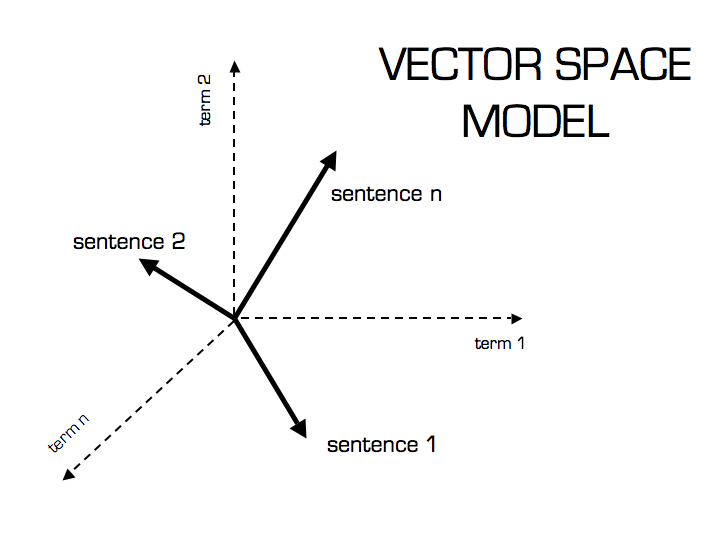
\includegraphics[width=0.7\textwidth]{vsm.png}
      \caption{"Vector space model"}
      \label{vsm_pic}
  \end{figure}

  \paragraph{}
    The vector space model in the text domain has the meaning that each word is a component of a vector resembling documents. If a document has 100 distinct words, the resulting document vector is in 100th dimensional space. If a second document has 50 distinct words, independant of the first document, both vectors are now in 150th dimensional space. That is, every new word will be concatenated to the existing document sets. This is the ``bag of words'' model which is detailed in the next section.

  \subsection{Notation}
    Before moving on we have to denote some notations and definitions. 
    A corpus $C = \{d_1, d_2 \: .. \: d_m\}$ is defined as a collection of \emph{documents} where $m = |C|$. A document $d = (w_1, w_2 \: .. \: w_i)$ contains words \emph{w} where $i = |d|$. Note that each document is not a text but a sequence of words. Often special stopwords are filtered out of these documents as well. A dictionary $D = \{w_1, w_2 \: .. \: w_n\}$ contains all the distinct words from each document where $n = |D|$. A cooccurence matrix $M$ is

      \[
        M=\kbordermatrix{%
              & w_1     & w_2     &  .. & w_n     \\
          d_1 & c_{11}  &  c_{12} &  .. &  c_{1n} \\
          d_2 & c_{21}  &  c_{22} &  .. &  c_{2n} \\
          ..  & ..      & ..      &  .. &  ..     \\
          d_m & c_{m1}  & c_{m2}  &  .. &  c_{mn}
        }
      \]

    where rows are the documents $d_1..d_m$ of a \emph{corpus} and columns are the cooccurence counts $w_1,w_2..,w_n$ of the corpus's dictionary. The next section \ref{sec:bag_of_words} explains this in more detail. Often the transpose $M^{T}$ is taken into account as well, setting rows to columns and columns to rows. Often the words are selected based on different feature selection strategies as well, see section \ref{sec:selection}. A distance matrix $Dis$ is defined as

      \[
        Dis=\kbordermatrix{%
              & d_1     & d_2      & ..  & d_m    \\
          d_1 & v_{11}  & v_{12}   & ..  & v_{1m} \\
          d_2 & ..      & v_{22}   & ..  & v_{2m} \\
          ..  & ..      & ..       & ..  & ..     \\
          d_m & ..      & ..       & ..  & v_{mm}
        }
      \]

    where each document is compared to another document by some similarity measure. See section \ref{sec:similarity} for more information. $v$ is any value that the distance function can incorporate.


  \subsection{Bag of words}
  \label{sec:bag_of_words}

    The bag of words assumption says that a corpus can be represented as a count or word occurence matrix. That means \emph{m} documents form a subspace in an \emph{m x n} matrix where \emph{m} denotes the corpus size and \emph{n} the dictionary of the words. Typically the assumption is binary, that is an occurence of word \emph{i} in a document \emph{j} is set to 1 else set to 0. Bag of words is also another way of saying that words are exchangable in order. That means the joint probability of N following words is equal to any of its permutations $p(w_1..w_N) = p(w_N..w_1)$, thusly leading to the assumption that the probability of a sequence of words can be viewed as a mixture over words. Later we will see this applied to the \emph{expectation maximization} algorithm.\\
    In reality this is not true, but without this assumption most of the models would be computationally expensive (up to unsolvable) and hard to reason about. In real world examples this is typically no problem but one has to account for the fact that indepedence of word sequences is a strong axiom that in reality is not true.

    \begin{table}[h!]
      \centering
      \begin{tabular}{c|c|c|c}
        \multicolumn{1}{r|}{} & \multicolumn{3}{c}{Words} \\
        \cline{1-4}
        Documents &   politics &   corruption &  policy  \\
        \hline
        document1 &    1 (2)   &     1 (1)    &   0 (0)  \\
        document2 &    1 (4)   &     0 (0)    &   1 (2)  \\
        document3 &    1 (1)   &     1 (6)    &   0 (0)  \\
      \end{tabular}\\
      \caption{"Document term (m x n) matrix"}
    \end{table}

    Normally we have a lower \emph{m} and a much higher \emph{n} resulting in highly sparse vectors with a lot of zeros, typically 99\%. As stated before we state that words are indepedant from each other. That means highly correlating words like \emph{New} and \emph{York} are not accounted for. In this case they can actually refer to the verb \emph{new} and \emph{York} as a city in \emph{Great Britain}. A bigram e.g. \emph{(New, York)} would capture the concept \emph{New York}. Bigrams, trigrams or generally ngrams are not taken into account. Ngrams transform a sequence of words by \emph{n} such that 

      \begin{equation}
        f(n = 2, (w_1, w_2, w_3) \in d) \to [(w_1, w_2),(w_2,w_3)]
      \end{equation}

    Adding ngrams to a document term matrix can greatly enhance similiarity between two documents. Keeping the dictionary and adding ngrams to the vector space results in \emph{n+(n-1)} memory requirements. If the data is already extremely sparse this will not help much but can increase the semantic effect on documents that share similar word combinations. There are other much more complex models e.g. \emph{noun phrases} or \emph{named entities} that can grasp this intuition as well. From a statistical point of view this is captured by collocations stating that certain word combinations occur more often than they would by chance occur. Therefore it is reasonable to assume that collocations are found in other documents as well strengthening the connection between two documents.

    The document term matrix can be enhanced by taking the count of the occuring words instead of just labelling it by occurence. This is called the raw frequency and can be normalized in a couple of ways by the term frequency (tf) model
     
      \begin{equation}
        f(t,d) = c
      \end{equation}

    where \emph{c} is the total count of term \emph{t} occuring in document \emph{d}.
    And a general term frequency function that helps against long document bias by normalizing with the maximum frequency of any occuring word in d.

    \begin{equation}
      tf(t,d) = 0.5 + \frac{0.5 * f(t,d)}{max(f(w,d)\, \forall w \in d)}
    \end{equation}

    The term frequency model can be further advanced by caculating the inverse document frequency (idf).

    \begin{equation}
      idf(t, C) = log(\frac{|C|}{|\forall d \in C : t \in d|})
    \end{equation}

    Where |C| is the size of the corpus and we check for every document in the corpus if the term occurs in the document. The intuition is: How often does a term occur in other documents. If a term appears more often then it is a common word such as ``the'', whereas ``super-symmetry'' might be a rare word. It is therefore some measure of importance. Because idf and tf only measure either importance accross all documents or importance of one document, we need to find words that are not rare and not common either. Generalizing the term-frequency and inverse-document-frequency we obtain the tf-idf:

    \begin{equation}
      tfidf(t, d, D) = tf(t, d) * idf(t, D)
    \end{equation}

    The tf-idf has a high score, if a term occurs often in a single document and less often in other documents. This translates to the notion that a term represents the current document better than other terms and are therefore highly discriminative words. There are other models such as graph based or tree based approaches. For the porpuse of this thesis these models are left out. \cite[chp. 6]{IRBook2008}\\

    One of the big problems with the vector space model is that feature inflation or feature explosion arises quickly. If documents have a high variance between other documents and the connections between two documents are small the sparsity can go up to 100\%. That means that no document has overlapping words and each document only accounts for the words that were originally in the document. Think of it another way, suppose one has 3 documents in 3 dimensional space with each axis set to zero but one (1,0,0), (0,1,0), (0,0,1) we have an independant basis. This means that all documents are orthogonal to each other, meeting at no point except at the null point (0,0,0). It is therefore not really possible to derive any connections between those 3 points. Thus each document represents its own topic.
    These kind of problems need a well thought out solution which is presented later in this section.

  \subsection{Similarity and Distances}
  \label{sec:similarity}

    \emph{Partitional clustering} algorithms commonly work through some objective distance or similarity function between two objects. After lifting the documents into vector space, we are faced with the problem of distance between two documents. Several measures were proprosed that can be easily interpreted by geometry or linear algebra. Our goal is to have an \emph{m x m} matrix for \emph{document x document} distances. A \emph{document x terms} matrix on the other hand is highly relevant when clustering under the assumption of topical classification. That is, compare documents not to each other but to all the occuring words as topics. \emph{Latent semantic analysis (LSA)} is a method where words are projected to lower dimensions by singular value decomposition. This resembles partial categorization to topics of a document by the most distinct words. Then a clustering can be done by documents that highly correlate to the same topics. See \ref{sec:lsa} for more information.

    \paragraph{The Cosine similarity} is a measure of orientation, not the magnitude. The angles between documents are compared and thus if the angle is $0°$ both documents are equal in size and word occurences. Given two documents $d_1$ and $d_2$ the classical cosine similarity is defined by

    \begin{equation}
      cosine(d_1, d_2) = \frac{d_1 * d_2}{||d_1|| * ||d_2||}
    \end{equation}

    If the documents are already defined unit vectors cosine similarity is just $cos(d_1, d_2) = d_1 * d_2$. Often we would like to consider the geometrical distance between two points taking the maginute of a vector into account as well.

    \paragraph{The Euclidean distance ($l^2\:norm$)} is the geometrical distance between two vectors in $\mathbf{R}^n$. Again given two documents $d_1$ and $d_2$ it is defined by

    \begin{equation}
      euclidean(d_1, d_2) = \sqrt{\sum_{i=1}^{M}(d_1^i * d_2^i)^2}
    \end{equation}

    This results in the fact that documents running into different directions, e.g. have different angles might as well be very close. It is a geometric measure and accounts for magnitude rather than direction.

    \paragraph{The Manhattan distance ($l^1\:norm$)} is commonly known under the city block distance measure. The system is divided up in equally squared brackets comparing dimensions in sequential order and taking the absolute squared difference between two documents. Given two documents $d_1$ and $d_2$ it is defined by

    \begin{equation}
      manhattan(d_1, d_2) = \sum_{i=1}^{M}|d_1^i - d_2^i|
    \end{equation}

    There are more distance functions such as the \emph{Jaccard coefficient} that works on intersections of sets and the \emph{Chebyshev distance} which is a maximizing greedy strategy of the manhattan distance. The underlying concepts of similarity should be clear though. Each coefficient works good on a particular set, however cosine and euclidean distances are the commonly used choices.

    \emph{Hierarchical algorithms} use different metrics. The goal here is not to find the closest points but to find the closest intersecting clusters. Hierarchical algorithms merge clusters based on linkage strategies. Those merges are seen as a split in the resulting directed acyclic graph. We will review them later as their functionality strays away from the vector space.

  \subsection{Enhancing the Vector Space Model}
  \label{sec:evsm}

    The vector space model comes with a variety of problems. First we have extremely high dimensions. As we see later this is particularly true for newspapers. Unlike Twitter the content of a newspaper article can be substantial and range over a variety of topics. This can lead to extremely poor clustering results. Several methods have been proposed to tackle this high dimensionality problem. One of the most strickening comes from linear algebra and was initially proposed in \cite{DeerwesterLSI1990} called Latent Semantic Analysis (LSA). It is based on Singular Value Decomposition (SVD). The Principal Component Analysis (PCA) on the other hand uses SVD in a different manner. Apart from these there are also much more elaborate techniques in the domain of topic modelling which will be reviewed later.

    \subsubsection{Latent Semantic Analysis}
    \label{sec:lsa}
      Latent Semantic Analysis is a progress to reduce as much noise as possible from a given term x document matrix to expose the so called latent variables. It is connected to topic modelling but seems to be more relevant in the context of dimensionality reduction. Dimensionality reduction is used for dealing with large sparse data to find the underlying connecting relations. \emph{LSA} is a truncated singular value decomposition \emph{(SVD)} on a term x document matrix. \emph{SVD} is a matrix decomposition where an n x m matrix \emph{A} is decomposed into three matrices $U$, $\Sigma$ and $V^{T}$. \emph{LSA} is constrained by the number of dimensions \emph{k}:

      \begin{equation}
        svd(A) = U_{mxm}\Sigma_{mxn} V^{T}_{nxn} \to lsa(A, k) = U_{mxk}\Sigma_{kxk} V^{T}_{kxn}
      \end{equation}

      While in the original \emph{SVD} we keep all components decomposing their respective singular values, \emph{LSA} only keeps \emph{k} components reducing the dimensions from \emph{n} words to \emph{k}. $\Sigma$ holds the k best singular values in sorted order. $V^{T}$ is a k x document matrix, where k are the reduced topics from the words. While we can do \emph{LSA} over documents, we can also use it for summarizations of single documents.

      \begin{figure}[h!]
        \centering
          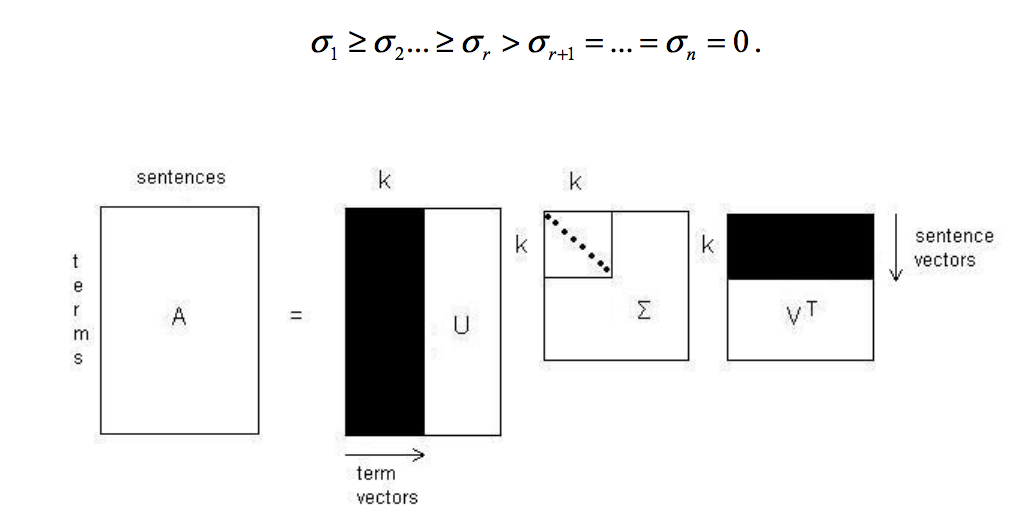
\includegraphics[width=0.7\textwidth]{svd_lsa.png}
          \caption{"Singular Value Decomposition by \cite{SumLSASteinberger2004}"}
          \label{svd_lsa}
      \end{figure}

      The $\sigma_1 \geq \sigma_2..\sigma_k$ stands for \emph{k} preceeding singular values sorted by magnitude. \emph{LSA} gives us a mapping from the top k topics of the document to the most important sentences of the document. In descending order the document presents less information per sentence. Thusly taking the top k sentences to create summarization can lead to significat results in a summarization processor. \cite{SumLSASteinberger2004}
      The intuition behind \emph{SVD} is to expose as much variance as possible at the same time reducing noise from the data. \emph{SVD} then is a natural progress to reduce highly sparse data projecting it to a lower dimensional space. This corresponce to a notion of topic overlap between different documents.
      Documents that share a particular topic are more similar. This results in connections between documents even if a lot of the words share no common meaning. Effectively \emph{LSA} tackles problems of synonymy and polysemy. Synonymy means that several words often share the same meaning such as ``big'' and ``large''. While polysemy refers to the fact that one word can have several meanings such as ``bank'' as a fincancial institution and ``bank'' as an object to sit on.

    \subsubsection{Principal Component Analysis (PCA)}
    \label{sec:pca}

    The \emph{Principal Component Analysis (PCA)} is a multivariate technique separating out correlating variables into principal components. \emph{PCA} in general is a dimensionality reduction technique reducing the number of features to a lesser set of features. The difference between \emph{PCA} and \emph{LSA} is the input. \emph{PCA} takes a covariance matrix $A*A^{T}$ which means that either only word x word or document x document matrices are taken as input. This makes it perfect for reducing dimensions after creating a cosine similarity matrix from the documents to visualize results.

    \begin{figure}[h!]
      \centering
        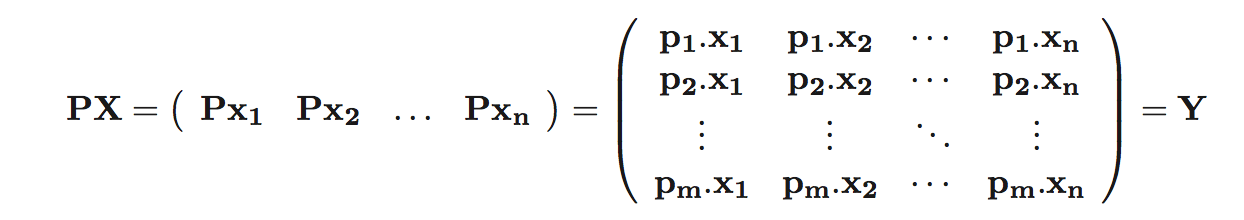
\includegraphics[width=0.7\textwidth]{PCA.png}
        \caption{"Principal Component Analysis by \cite{PCA2009}"}
        \label{pca}
    \end{figure}

    In figure \ref{pca} we find the \emph{n} most likely components of a document by decomposing an original document matrix $X$ by factoring out $P$ principal components. The input is no $n\:x\:m$ matrix but rather a covariance matrix $n\:x\:n$ or $m\:x\:m$ . These components capture the variance throughout each document individually and reduce the dimensions down to a specified \emph{k}. The factorization then tries to solve for a principal component that bestly resembles the original data. In practice \emph{PCA} is conversion of a document by term matrix into a covariance matrix followed by \emph{SVD} where principal components resemble the highest singular values up to $k$. Primarily \emph{PCA} can be described as a dimensionality reduction technique that resembles the original structure well. It can be used for visualization, reducing down $n + 3$ dimensions to 2D or 3D. See more in \cite{PCA2009}.

\section{Clustering algorithms}
\label{sec:clustering}
  
  Clustering algorithms are the procedures, describing, how data can be automatically assigned to groups by similarity metrics. They are unsupervised methods and can be combined by explicit knowledge engineering. They come in shape of \emph{partitional} models, that flatten the structure, in \emph{hierarchical} models that build tree like structures, \emph{spectral} algorithms that are \emph{graph based} or \emph{density} based algorithms. There is also a fifth category namely \emph{generative models} and closely related in terms of the text domain \emph{probabilistic topic models}. These models try to find the underlying latent semantics by generating the model that could have created the documents in the first place. First let us setup a few definitions that all clustering algorithms incorporate.

  \begin{itemize}
    \item \emph{Hard and Soft clustering} - A clustering algorithm is \emph{hard} if documents can only be assigned to one distinct cluster. On the contrary they are \emph{soft} (often called \emph{fuzzy/overlapping}) if a document can have multiple assignments that resemble topical proportions of the document.
    \item \emph{Exhaustive and non-exhaustive} - A clustering is exhaustive if every document has an assignment after the run whereas it is non-exhaustive if documents might not have any assignments at all (assigned to a null cluster).
    \item \emph{Cost functions} - Most clustering algorithms incorporate some sort of cost function that needs to be minimized or maximized after the algorithm completed. The clustering can be rerun several times finding a maximum between different runs by varying the parameters. This should not be confused with the similarity measure between objects during a clustering run.
    \item \emph{Local minima/global optimum} - A local minimum is when the objective cost functions between objects do not yield better results after several iterations. This does not mean that the best state is found. Similarity metrics between objects are inherently heuristic and have no view of a global optimum. A global optimum can be approximated by objective cost functions rerunning the algorithm several times. There is currently no known algorithm that can solve clustering in a deterministic globally optimized way.
  \end{itemize}

  \subsection{Partitional clustering}
  \label{sec:partitional}

    \emph{Partitional clustering} algorithms build up centroids. They resemble typical cluster centers. After documents are converted into vector space and some sort of similarity measure is applied, cluster centers are incrementally created. We briefly review two partitional clustering algorithms namely \emph{K-Means} and \emph{Expectation Maximization (EM)}. Literature in this area is rigorous, see \cite{ClusteringBooAggarwalk2013, NextFrontierClustering2013, IRBookStanford2008}.

    \begin{figure}[h!]
      \centering
        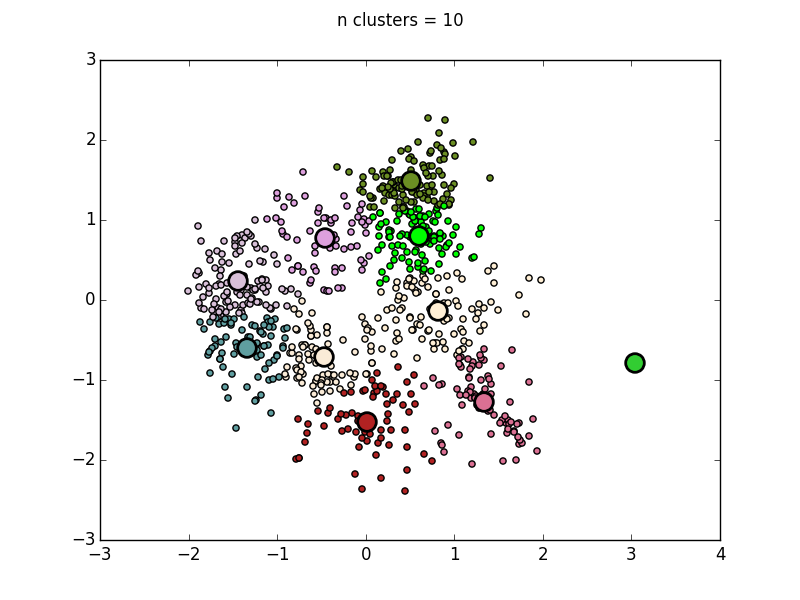
\includegraphics[width=0.7\textwidth]{kmeans_clustering.png}
        \caption{"K-means visualisation with applied dimensionality reduction"}
        \label{kmeans_clustering}
    \end{figure}

    Figure \ref{kmeans_clustering} is a typical clustering result. Note: to display 2D models one has to use dimensionality reduction techniques reducing the feature size. The original dataset consisted of over 100k words so this is a rather unfair approximation of the original dataset. The larger points correspond to cluster centers while the smaller points correspond to individual documents adhering to the cluster centers colors. \\

    \emph{Partitional clustering} algorithms typically have linear running times and thus are often used in practical real world applications. We will see later that this comes with a price mostly in accuracy and by providing the number of clusters. Most of the time we do not know how many clusters will be in the final result so we need algorithms that can find an approximately optimal clustering. In particular partitional algorithms can be globally approximated given a numerical cost function $f:D \to \mathbf{R}$ such that it maximizes $f(d_i) \geq f(d_j), \forall d \in D$  or minimizes $f(d_i) \leq f(d_j), \forall d \in D$. Often they are much easier to implement because constraints are kept low and requirements are kept to a minimum. $d_i,d_j$ are all pairs of documents in a collection of documents $D$. There are also online versions available which make it possible to scale algorithms such as K-means with \emph{map reduce} on several processors. This is not true for hierarchical algorithms that build up a hierarchy bottom-up or top-down. The difference is that partitonal algorithms assign to cluster centers, while hierarichal algorithms build up pairs of merges, resembling a merge tree. This makes it difficult to scale hierarchical algorithms as they need a global picture of distances to be generated.

    \subsubsection{K-Means}
    \label{sec:k_means}

    The \emph{K-Means} clustering algorithm is a centroid based algorithm. Each document is assigned to a cluster center in each iteration. In order to do this \emph{k} centroids are drawn as a initial cluster centers from the documents. Then interdistance similarity measures, typically $l_2\:norm$, decide if a document is closer to a certain centroid. Centroids will be moved to the new location in vector space by averaging over the assigned documents. In the next iteration a document then might be reconsidered for another cluster. \emph{K-Means} typically forms clusters of equal sizes and is a hard clustering algorithm \cite{IRBookStanford2008}.\\
    Typically a \emph{K-Means} algorithm will be run with respect to an objective cost function to be minimized. Globally this can be used for chosing a suitable \emph{k} for the underlying data. The objective goal is to minimize the residual sum of squares of within cluster distances \cite{IRBookStanford2008}:

      \begin{equation}
        RSS_k = \sum_{\vec{y}_k \in \textit{w}_k}|\vec{y} - \vec{f}(\textit{w}_k)|^{2}
        \label{RSS}
      \end{equation}

    If we now sum over all $RSS_k$ the total amount must be minimized. Formula \ref{RSS} is a vectorized form, where $y$ is a prediction column and $f(w_k)$ is the prediction given the assignments $w_k$ where $f$ is some kind of distance function. The algorithm converges either after not improving above a \emph{threshold} or by limiting the iterations by a paramter \emph{max iter} after which the algorithm stops. In this case both criterias are modelled which resembles the implementation by \cite{ScikitLearn} in Sklearn.

    \begin{algorithm}[H]
    \begin{algorithmic}[1]
      \caption{$X$ is a document term matrix, $\mu$ is a matrix of centroid vectors, $c$ a mapping between $X$ and $\mu$}\label{kmeans}
      \Function{Kmeans}{$X={x_1,..x_m},k,maxiter$}
        \State $\mu \gets select\:k\:initial\:centroids\:from\:X$
        \State $c \gets init\:assignment\:matrix {}$
        \State $cost \gets \infty$

        \For{$i\gets 1, maxiter$}
          \State $c \gets argmin|\vec{\mu} - \vec{X}|$ \Comment{assign X to k nearest centroids}
          \State $\mu \gets average\:X\:over\:assigned\:\mu\:by\:c$
          \State $cost \gets \sum_{n = 1}^{k}RSS_k$
          \If{$cost\:lead\:to\:convergence$}
            \State Stop
          \EndIf
        \EndFor
        \State \Return $labels, centroids, cost$
      \EndFunction
    \end{algorithmic}
    \end{algorithm}

    \emph{Now we are left with one problem}: How do we choose the initial clusters? Several strategies have been proposed. The most used is random sampling where \emph{k} random documents are chosen as a centroid. The problem is, when all documents are skewed to one direction or close together the \emph{K-means} converges at a local minimum that seems to suboptimally divide the documents into clusters.
    Another strategy has been proposed by \cite{KMeansPlusPlus2007} that maximizes the intercluster distance by spreading the clusters as far from each other as possible. 
    As the initial clusters are often picked randomly \emph{K-Means} is a non deterministic approach that will most likely result in different clusters after each run.

    \subsubsection{Expectation Maximization (EM)}
    \label{sec:em}

    The \emph{Expecation Maximization (EM)} algorithm is a generalization of \emph{K-Means} and a soft clustering algorithm with fuzzy associations between clusters and documents. The underlying methodology is that we would like to find a model that generated the given documents. The way this works is first by assuming that the clusters are represented as random distributions over terms. They can be assumed as a normal gaussian distribution. Note: the kind of distribution can vary, gaussian distributions can tend to zero if no assignment was found and so EM could assign no label at all. If that is not desired and a soft and exhaustive clustering is prefered one can add additive smoothing, that other models like the Dirichlet model inheret. What we would like to know is: How does a data point \emph{x} relate to the different \emph{k} guassian distributions? Formally we need to estimate a model $\Theta$ that is maximized using a cost function such as \emph{maximum likelihood estimation (MLE)} given some data. The intution is, by estimating the likelihood of a given incomplete dataset $D$, that is assumed to be normally distributed, we want to maximize the connection between $\Theta$ and $D$.

      \begin{equation}
        \Theta = argmax\:\sum_{n=1}^{N}log\:P(d_n,\Theta)
      \end{equation}

    Where $P$ is the fractional probability that a document $d_n$ was generated by $\Theta$. In the text domain this means: for all words in each $D$ can we generate assignments to distributions that maximize $\Theta$.
    The \emph{EM} algorithm tries to maximize this function by assigning a probability that a data point $x$ is likely to be in the cluster $c_1..c_k$ by calculating the joint probabilities of occuring words given a prior of cluster $c_1..c_k$. This is also called the expectation step. In the second step each probability of a document \emph{d} being part of a cluster $c_1..c_k$ is weighted into the average and variance of the defined clusters. The clusters are then recalculated using the beforementioned assignments. This step is repeated until some kind of convergence criteria has been met. The main intuition is if we have a model $\Theta$ we can compute the fractional probabilities of a document $d$ to be in a cluster $k$:

      \begin{equation}
        P(d|\Theta) = \sum_{k=1}^{K}\alpha_k\left ( \prod_{t_m \in d} P(t_m = 1|c_k) \right ) \left ( \prod_{t_m \not\in d} (1 - P(t_m = 1|c_k)) \right )
      \end{equation}

    In the maximization step we then need to compute the probability that a term $t_m$ has a high probability to be in $c_k$ that is $P(t_m = 1|c_k)$ and the prior $\alpha_k$ that is the probability that any document is in $c_1..c_k$ given no evidence. In the expectation step we compute $r_{nk}$ that is the soft assignment of a document $d_n$ to a cluster $k$. $r_{nk}$ is computed with the soft assignments of the prior $\alpha_k$ and $P(t_m = 1|c_k)$.\\
    The inherent problem remains: How do we choose $\alpha_k$ and $P(t_m = 1|c_k)$? $\alpha_k$ and $P(t_m = 1|c_k)$ are needed to recompute the soft assignments. At the beginning assignments are assumed to be randomly mixtured. After several iterations documents are weighted into the initial random selection until convergence. So to speak the documents contribute to the model over time up until no change has been seen to the iteration before. For further information see \cite{IRBookStanford2008}. Later we will discuss the generative models more indepthly. The \emph{EM} algorithm can work with a lot of distribution. Like the Gaussian distribution, we can work with other multinominal distributions assuming different priors.

  \subsection{Hierarchical / Agglomerative clustering}
  \label{sec:hierrachical}

    \emph{Hierarchical agglomerative clustering (HAC)} algorithms build up hierarchies of clusters with  documents on their leaf nodes. There are two approaches available. By bottom-up, assuming all documents to be clusters, agglomerating them upwards until a root node has been found. Or by top-down, starting with all documents in a cluster, splitting them down until the leafs are documents. Often we can constrain this process by limiting the cluster size as well. Then \emph{HAC} first clusters document to create a tree and then later cutting the tree by heuristics such as a given cluster size k or by a distance threshold. It is a big discussion in the scientific community if hierarchical clustering as opposed to partitional clustering algorithms give better results. \cite[chp. 17]{IRBook2008}\\
    \emph{HACs} typically have higher runtimes due to the fact that most of them infer the count of clusters and build up a hierarchy until convergence. The runtimes are often in $O(N^2)$ or $O(N^3)$. As seen below in figure \ref{hac_dendogram} hierarchical clusterings can be easily visualized as dendograms. Dendograms show a history of the merges of different clusters up to the root nodes.

    \begin{figure}[h!]
      \centering
        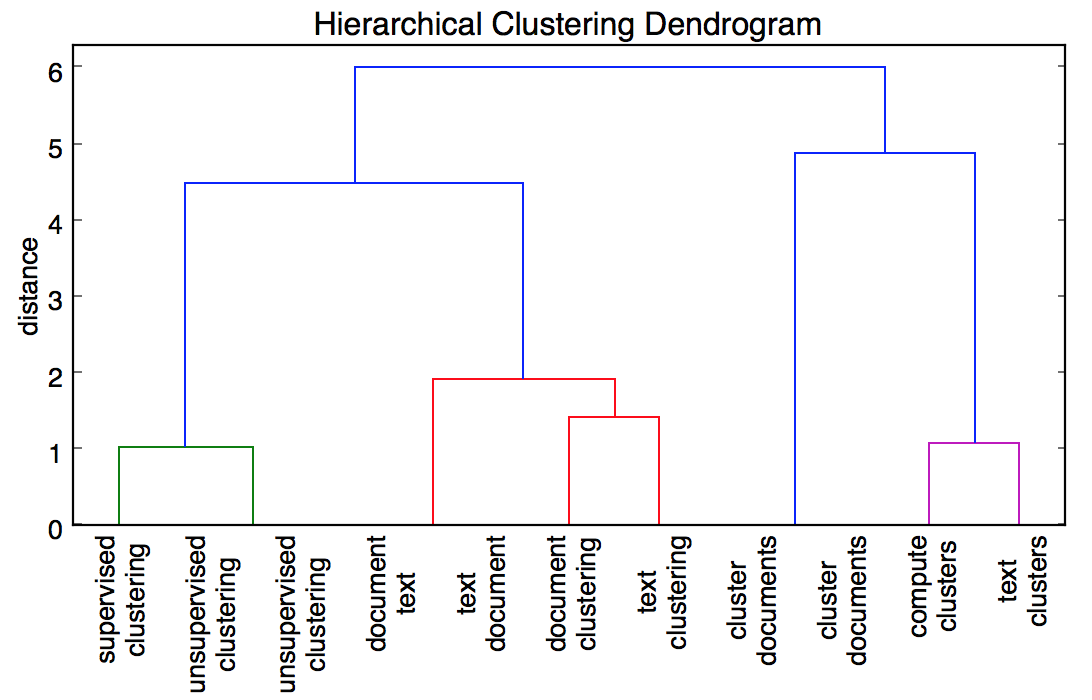
\includegraphics[width=0.7\textwidth]{dendogram.png}
        \caption{"Ward linkage dendogram"}
        \label{hac_dendogram}
    \end{figure}

    On the \emph{y} label there are decreasing distances. The \emph{x} label presents the leaf nodes where at most two documents are paired to each other. For instance ``unsupervised clustering'' occurs twice so the distance between these two is 0. While at the same time ``supervised clustering'' seems to be close. The merge one hierarchy up could resemble a cluster where the 3 documents resemble one bigger cluster. The distance at the \emph{y} level is monotonically increasing bottom up. Each successive merge must be at a higher distance than the merge before. By threshold, distance density or a fixed cluster size k, we can form clusters at different granularities. To start hierarchical clustering a $m\:x\:m$ distance matrix has to be created. The closest two documents will be iteratively merged until no unassigned document remains. Keeping track of the merging processes in each iteration can be seen as overlapping clustering centers.\\

    A simple \emph{HAC} scheme first finds the maximizing next distance between two documents that have not yet been merged. Then these maximized document pairs $d_1$ and $d_2$ will be merged resulting in a new higher level merge. The similarity in \emph{HACs} are stated by linkage criterias. The question then is: given two merges $c_1,c_2$ how can we compare them?

    \begin{algorithm}[H]
    \begin{algorithmic}[1]
      \caption{$D$ is a document term matrix}\label{hac}
      \Function{HAC}{$D={d_1,..d_m}$}
        \State $C \gets initialize\:m\:by\:m\:distance\:matrix\:over\:D$
        \State $I \gets list\:of\:length\:m\:I[m]=1$ \Comment{List of unmerged documents}
        \State $H \gets \{\}$ \Comment{History of merges}

        \For{$k\gets 1, m$}
          \State $g \gets \{i\not=l \wedge I[i]=1 \wedge I[l]=1 \}$
          \State $i,l \gets  argmax\:\{ i,l : g\} C[i][l]$ \Comment{Return maximized indices over C}
          \State $H \gets (i,l)$ \Comment{Keep track of merges}
          \For{$j\gets 1, m$} \Comment{Update C with respect to all other clusters}
            \State $C[i][j] \gets LinkageSim(C[i][l], C[l][j])$
            \State $C[j][i] \gets LinkageSim(C[i][l], C[l][j])$
          \EndFor
          \State $I[l] \gets 0$ \Comment{Deactive from active clusters}
        \EndFor
        \State \Return $H, C$
      \EndFunction
    \end{algorithmic}
    \end{algorithm}

    \subsubsection{Linkage strategies}
    \label{sec:linkages}

    In the following we will explore some of these different linkage clustering strategies.
    The refered to distance function will be one of the conventional distances such as \emph{cosine} or \emph{euclidean}.

    \paragraph{Single linkage} takes two documents of the corresponding clusters $c_1,c_2$ that minimizes the distance between these two. The objective function corresponds to:
      
      \begin{equation}
        \forall d_1 \in c_1 \wedge \forall d_2 \in c_1: min(distance(d_1, d_2))
      \end{equation}

    In figure \ref{linkage_strategy} we can see that single linkage takes, geometrically, the two clostest points of $c_1,c_2$. It is single in a sense that no other documents are considered but the closest two.

    \paragraph{Complete linkage} takes two documents of the corresponding clusters $c_1,c_2$ that maximizies the distance between these two. The objective function corresponds to:
      
      \begin{equation}
        \forall d_1 \in c_1 \wedge \forall d_2 \in c_1: max(distance(d_1, d_2))
      \end{equation}

    In figure \ref{linkage_strategy} we can see that complete linkage takes, geometrically, the two farthest points of $c_1,c_2$. It is complete in saying that it is not underestimated by taking the high variance into account.

    \paragraph{Average linkage} takes all documents of the two corresponding clusters $c_1,c_2$ and averages them with all corresponding clusters. That is we take all documents into account and link them by their average. The objective function is:

      \begin{equation}
        \frac{1}{|c_1|*|c_2|} \sum_{d_1 \in c_1} \sum_{d_2 \in c_2} distance(d_1, d_2)
      \end{equation}

    In figure \ref{linkage_strategy} we can see that average linkage takes the average of all documents in a cluster and calculates the distance between both averages.

    \begin{figure}[h!]
      \centering
        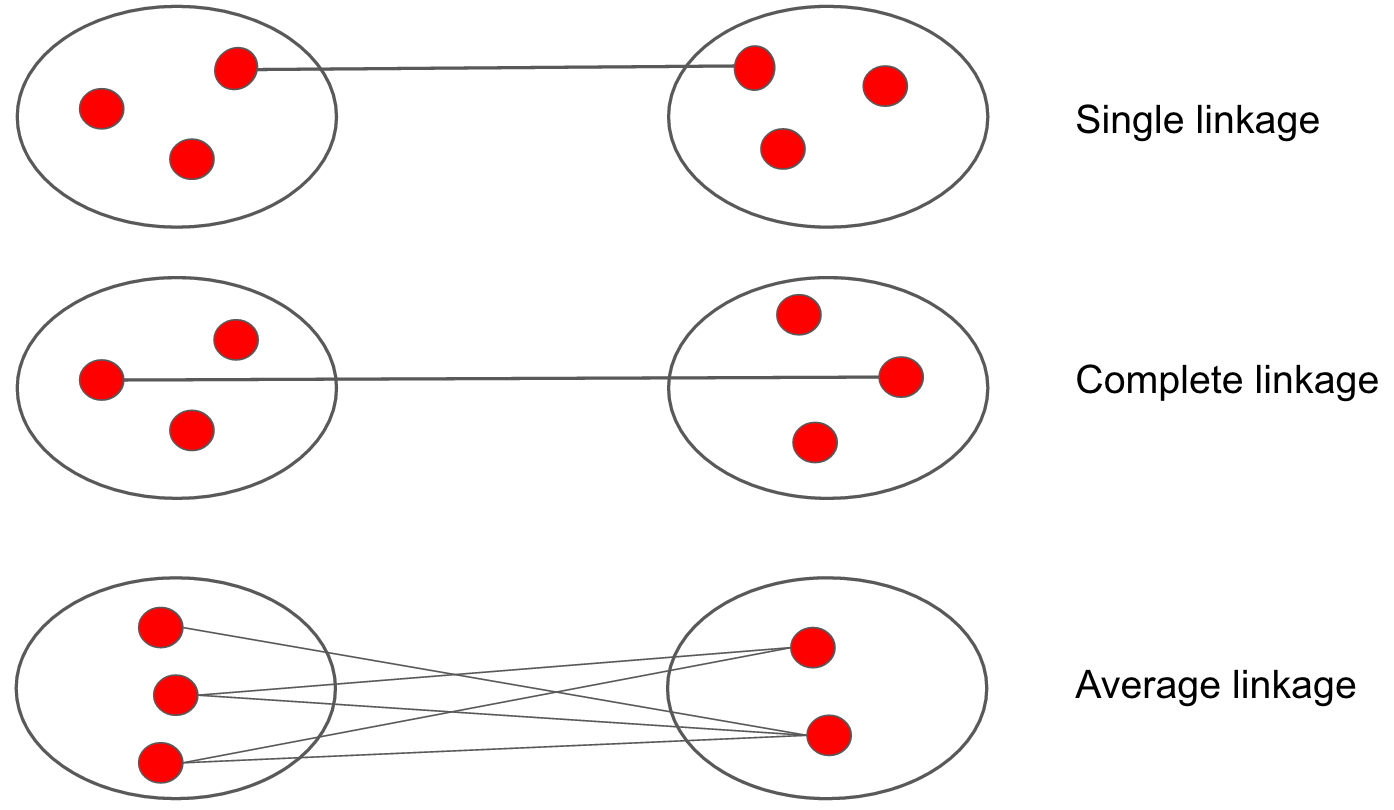
\includegraphics[width=0.7\textwidth]{linkage_strategy.png}
        \caption{"Single, complete and average linkage"}
        \label{linkage_strategy}
    \end{figure}

    There are other strategies such as centroid based, Wards method and minimum energy based.
    All strategies have different purposes and have their place. Single linkage might be best suited for problems where the data points are dense and not scattered throughout the vector space. Complete linkage might work well if data is scattered widely in high maximas so to approximate an ideal solution. Average linkage would overestimate these cases by too many outliers. On the other hand average linkage is the best choice if documents are assumed to  participate equally. 
    \paragraph{Birch} is a specialized version of \emph{HACs}. It scales well to large datasets and is an incremental algorithm. It operates in different phases and can be constrained by an optional cluster size \emph{k}. One can provide parameters for maximum nodes per cluster and minimum density threshold as to when a document should be assigned to a cluster. See 
    \cite{BIRCH1996} for more information. As with the partitional algorithms this was studied extensively by \cite{ClusteringBooAggarwalk2013, ClusterAlgoSurveyIBM, IRBook2008}. Top down approaches are not of special interest here. They are primarily suitable for large scale topic browsers where linear time constraints play a role.

    \subsection{Generative Models}   
    \label{sec:generative}

      According to \cite[Wikipedia]{Nothing} a generative model is a model for randomly generating observable data values, typically given some hidden parameters. It specifies a joint probability distribution over observations and label sequences. In the area of document clustering and text summarization they play a role in modelling documents by word distributions assigned to topics. The \emph{EM} algorithm is a typical scheme of a generative model, found in the partitional clustering section. In the text domain, topic modelling plays an increasing role for identifying latent topics from a distribution of documents and words. By \emph{bayesian inference} we can draw conditional probabilities from word to document to topic proportions. Making sense of these quantities is part of probabilistic topic modelling. As with the \emph{EM} algorithm we draw partial probabilities that a document was generated by a mixture of topics. Several widely used methods namely \emph{Latent Dirichlet Allocation (LDA)}, \emph{Hierarchical Dirichlet Process (HDP)} as well as the beforementioned \emph{Latent semantic analysis (LSA)} are found in the generative realm. Usually, generative models are too expensive for large datasets. That is why most of the algorithms use variational inference resulting in the possibility to use online algorithms.

      \subsubsection{Topic modelling}
      \label{sec:topic_modelling}

        Probabilistic topic modelling is a generative approach where documents are assumed to be mixtures of topics. A topic is a mixture of words describing probabilities how much a word constitutes to a topic. The underlying question then: Given a set of documents $D$ and given random topic mixtures $Z=\{z_1..z_k\}$ what words $w_1..w_n$ of a particular document $d$ constitutes to which topic. Given a document $d$ with words $W=\{w_1..w_n\}$ and some mixtures over words $Z$ how often does a particular word from $W$ occur in topic $Z$. Further how common is topic $Z$ in the current document $d$. In the following we will briefly discuss topic modelling and its applications. See \cite{TopicModelsBlei2012}. The very basic form of topic models are drawn from multinominal mixtures over word proportions. We would like to know, given a document $d$ and some topics $Z$ how likely is it that a specific topic $z$ generated $d$?

          \begin{equation}
            p(d) = \sum_{Z} p(z) \prod_{w\:\in\:d}p(w|z)
          \end{equation}

        $p(z)$ is the probability that a random document is part of that topic distribution and $p(w|z)$ is the conditional probability that given a word $w$ evidenced by $z$, how likely is it to be drawn? This tones down to bayesian inference. We quickly see that in this process each document is drawn with the priors $p(z)$. Further each document gets hard assignments, a document is matched with a probability for a topic $z$. Statistical learning via \emph{EM} is required for all of these algorithms by drawing probabilities that estimate the maximum likelihood that a document $d$ is assigned to a topic $z$. The topic proportions need to be learned and so each document increments the parameter size to be estimated.

        \paragraph{Bayesian inference}
          In bayesian inference one would like to know, given some evidence how likely is it that some event happens? You would like to know given some event A, evidenced by B, how probable is A? In order to do so we have to take the prior of $P(A|B)$ that is the probability that some event $A$ without any evidence is likely, called $P(A)$. Multiply it by the probability $P(B|A)$ that is the reversed probability of $P(A|B)$ dividing by the probability of evidence $B$, $P(B)$.

          \begin{equation}
            P(A|B) = \frac{P(A) * P(B|A)}{P(B)}
          \end{equation}

          See \cite{Nothing} for a great introduction.
        
        The definition of a prior or prior distribution is important. A prior is a raw distribution over the outcomes of some event $A$, \emph{without} any evidence $B$. It is knowledge that needs to be observed. If no observations took place, we have to assume, beforehand, that the prior is randomly distributed. The generative process then weights in the words of each document and approximates the prior distributions. In the context of topic modelling, priors are topic distributions over words or documents.\\ 
        
      \subsubsection{Probabilistic latent semantic indexing (PLSI)}
      Advancing on the above statement, \cite{PLSA2001} created the \emph{probabilistic latent semantic indexing (PLSI)}.

        \begin{equation}
          p(d, w_n) = p(d)\sum_{Z} p(w_n|z)\:p(z|d)
        \end{equation} 

      \emph{PLSI} takes into account that words contribute to a topic. Documents are sequences of words, so a document can contain several topics as well. The assumption: A topic generated a specific word, so a document was generated by several topics. This is done by drawing $p(d)$ as before with the additional probability $p(w_n|z)$ that a word $w_n$ of a document $d$, evidenced by $z$ and $p(z|d)$ the most likely probability that a topic is drawn evidenced by $d$. Informally for each word $w_n$ in a document $d$ how likely was it generated by a topic $z$ given a document $d$.

      \begin{algorithm}[H]
      \begin{algorithmic}[1]
        \caption{probabilistic latent semantic indexing}\label{PLSI}
        \State $Choose\:a\:document\:d_m\:with\:p(d)$
          \For{$w_n \in d_m$}
            \State $z_n \gets multinominal\:from\:d_m\:p(z|d_m)$
            \State $w_n \gets multinominal\:from\:z_n\:p(w|z_n)$
          \EndFor
      \end{algorithmic}
      \end{algorithm}

      As seen in algorithm \ref{PLSI} the underlying problem is that topic distributions must be estimated for each document $d_m$ and for each topic $z_n$. This can be mitigated by using priors for topics instead of parameter estimations by \emph{EM}. For this reason \emph{Latent Dirichlet Allocation (LDA)} was proposed by \cite{LDA2003} where a Dirichlet prior is assumed before hand. For completeness the two models are briefly described.

      \subsubsection{Latent Dirichlet Allocation (LDA)}
      \label{sec:lda}

        Latent Dirichlet Allocation created by \cite{LDA2003} is \emph{PLSI} assuming a Dirichlet prior. Dirichlet distributions are often used as prior distributions in Bayesian statistics. The Dirichlet distribution is the conjugate prior of the categorical distribution and multinomial distribution. Its probability density function returns the belief that the probabilities of $k$ rival events are $x_i$ given that each event has been observed $\alpha_i-1$ times. \cite[Wikipedia quote for Dirichlet processes]{Nothing}\\
        This fact comes in handy especially when assuming that \emph{LDA} should generate $k$ distinct topic distributions over words that can be mapped to a topic distribution over documents. \cite{TopicModelsBlei2012}

        \cite[TODO: formulas and explanation]{Nothing}

        Alternatives to this are more complicated models like the \emph{Hierarchical Dirichlet Process (HDP)} by \cite{HDP2006} that can automatically infer the size of the topics or the \emph{Pachinko allocation} creating a hierarchy with directed acyclic graphs (DAGs). \cite{NonParametricBayes2007}
        
      \cite[Sum it up in a few words]{Nothing}

    \subsection{Others}
    In the literature there are a lot more strategies involved how clustering can be done. Often they are particulary good in specific domains such as images. In the text domain however they have high runtimes and are often not desirable in their output. They often lack good strategies to work with high dimensionality. We briefly note them here.

      \begin{enumerate}
        \item \emph{Spectral} - these are graph based algorithms. Distances are based on graph partitioning problems, where shortest paths, min cuts and graph partitions are used to define clusters. These problems are perfect for small document groups and are often used as subcluster procedures.
        \item \emph{Density} - these algorithms try to find documents that are within a certain distance to each other. Often one needs to provide density thresholds or neighboorhood graphs that determine how two documents should be grouped. From a geometric point of view, we would like to cluster documents that are within a certain distance radius. These algorithms are locally aware in that they do not care about a global optimization.
        \item \emph{Grid} - the vector space of the documents is split into equally sized grids. We then compute the density of the grids and identify the maximizing grids. Then the problem to cluster each document to a distinct cluster is based on graph traversal techniques. The intuition is that we do not consider single points but rather the surrounding grids.
      \end{enumerate}

    There are indepth studies on spectral, density and grid based algorithms in \cite{ClusteringBooAggarwalk2013}.


\section{Cluster evaluation}
\label{sec:evaluation}

  In order to comprehend if a clustering result is reasonably good or bad, we need to evaluate them. This can be done by purely mathematical formulas that output numbers a human expert can interpret or by displaying intuitive results via plots, topic browsers or text. The second category is highly subjective to the reviwer, while the first, at least, holds some objective criterias. Evaluation is a black art. Clustering itself has no real goal in terms of the domain. The primary goal is to group similar and dissimilar data points. What similarity and dissimilarity actually means is an open topic. All results of evaluation metrics need to be analysed and interpreted, otherwhise its numbers. High numbers can correspond to dense clusters, low numbers can correspond to scattered clusters. The actual numbers only make sense compared to what the domain needs to be solved.\\
  Formally we have two groups of measurements, the internal measures and the external measures. Going ahead a bit for the sake of this thesis we will use the \emph{purity}, \emph{V-measure} and \emph{silhouette coefficient} for evaluation of clustering results.

  \subsection{Internal measures}
  \label{sec:internal_measures}

    Internal measures describe how well a clustering result represents the original data. By mathematically evaluating the final intra cluster distances between the documents and their respective clusters and by calculating the dissimilarity between documents and other clusters. What we will find is that internal measures are often not suitable in asking about the quality of clusterings. Higher dimensionalities might lead to much better clustering results in a few cases, because the original data has a high variance. Internal measures on the other hand have better scores if the dimensions are lower. Using \emph{LSA} reducing the dimensions down to 1 will lead to extra ordinary high scores. The results of internal measures can thusly only be compared to other clusterings of the same dimensions. As there are several measures that can be employed for internal clustering evaluation we will briefly look more closely at the silouhette coefficient. There are other measures as well, for completeness they are shortly reviewed.

    \paragraph{The silhouette coefficient} is a measure for how dissimilar a document $d$ is to its own cluster $C_d$ and how dissimilar a document $d$ is to the closest neighbouring cluster in $C_{d \not \in C}$. Often denoted as $a(d)$ it is the average dissimilarity from $d$ to all other documents in $C_d$ and $b(d)$ picks the minimum dissimilarity of $d$ to all clusters $C_{d \not \in C}$. Then the silhouette of a document $d$ for a clustering $C$ is defined as

      \begin{equation}
        s(d, C) = \frac{b(d, C_{d \not \in C}) - a(d, C_d)}{max(\:b(d, C_{d \not \in C}), a(d, C_d)\:)}
      \end{equation} 

    The coefficient is 1 if the dissimilarity $a$ is low and dissimilarity $b$ is high, meaning $d$ is well clustered into $C_d$. Near to 0 if both are fairly equal, which means $d$ could fit into the neighbouring cluster almost as good as $C_d$. Finally -1 if the clustering went bad and $d$ is falsely assigned to $C_d$ whereas it should have been assigned to its neighbour. See \cite{Silhouettes1987} for detailed explanations.

    \paragraph{The Davies–Bouldin index} is a measure of distance between assigned intra cluster distances and inter cluster distances. That is a clustering is best if there is low intra cluster distance and high inter cluster distance to all clusters. A smaller value means better clustering. See \cite{DavisBouldin1979} for detailed explanations.

    \paragraph{The Dunn index} minimizes the distance between two clusters $c_1$ and $c_2$ with a variety of possible distance metrices such as average, maximum or euclidean and divides it by the maximized intra cluster distances. Thus the Dunn index is like the Davies-Bouldin index a measure of intra cluster compactness and inter cluster variance. See \cite{DunnIndex1973} for detailed explanations. 

  \subsection{External measures}
  \label{sec:external_measures}

    External measures describe how well a clustering performed provided with a ground truth of the documents. We often refer to this as the golden standard where human labellers assigned concrete classes to documents. With newspaper articles this is often the category of the article, like politics or business. Clustering results are measured by their ratios of labels to clusters and clusters to labels. The question that arises is: why use clustering for any kind of grouping in the first place if we already have class labels for the documents? This is adressed by only labelling a few documents of the original dataset and is called the training set. While this tackles the issue of spending time for labelling other problems arise. In clustering for summarization our inherent goal is not to group documents that necessarily share a label. Maybe we are interested in groups of documents that share proportions of labels as well.\\
    What we are mostly interested in are metrics that faciliates the notion of facts and predicition accuracy. The problem with clustering is that we do not know what the clusters actually mean. Before we can compare them to their respective labels we need to know for each cluster how documents were labeled. By counting all the occurences we can infer if documents were grouped into clusters with the same labels. If this is not the case then the labels either were not accurate enough or were accurate but the structure of the documents could not capture the assumptions. Generally we would like a high true positive score, meaning most of the documents that share the same label were in the same cluster. While at the same time maintaining a false positive score, meaning documents assigned to the wrong clusters. Wrong however seems relative if we are really not interested in a hard labelled clustering.

    \paragraph{Purity} is a basic score and facilitates the rate between correctly predicted results in relation to false results. Formally:

      \begin{equation}
        \frac{True\:Positives}{True\:Positives + False\:Positives}
      \end{equation}

    It is the ratio between all correctly predicted results the examples that were assigned into the correct cluster \emph{true positives} as a ratio to those that were falsely assigned to another cluster \emph{false positives}. A High purity indicates low error ratio in the False positives. This only accounts for the false and true assignments. But what is about labels that are partially in all clusters? We have to account for the variance how labels are spread too. It is actually worse if we have 5 clusters and 5 labels and one label is partially found in all 5 clusters how can we account for that?

    \paragraph{V-Measure} is an entropy based measure. It relies on the homogeneity score that measures if all of the clusters $c_1..c_k$ contain documents that are labelled with the same class and completeness score that measures if all documents that are members of a class are elements of the same cluster. Completeness and homogenity run in opposite directions. Informally if all points are in a single global cluster, then all classes are part of the same single cluster, thusly generating a high completeness score and a low homegeneity score. If each document is assigned to its own cluster, having as many clusters as documents, the homogeneity score is very high and the completeness score extremely low. The V-Measure then favours solutions where classes are assigned to a correct cluster (completeness), while keeping the classes distinct between clusters (homgeneity) \cite{VMeasure2007}:
      
      \begin{equation}
        homogeneity = 1 - \frac{H(C|K)}{H(C)}\\
        completeness = 1 - \frac{H(K|C)}{H(K)}
      \end{equation}

    where $H(C|K)$ is the conditional entropy of the classes given the cluster assignments (similary for completeness, change the conditional probability):

      \begin{equation}
        H(C|K) = - \sum_{c=1}^{|C|} \sum_{k=1}^{|K|} \frac{n_{c,k}}{n}\cdot \log\left(\frac{n_{c,k}}{n_k}\right)
      \end{equation}

    and $H(C)$ is the entropy of the classes:

      \begin{equation}
        H(C) = - \sum_{c=1}^{|C|} \frac{n_c}{n} \cdot \log\left(\frac{n_c}{n}\right)
      \end{equation}

    \cite{VMeasure2007} then define the V-measure as the harmonic mean of homogeneity and completeness:

      \begin{equation}
        v = 2 \cdot \frac{h \cdot c}{h + c}
      \end{equation}

    \paragraph{Adjusted Rand Index} - The Rand Index computes a similarity measure between two clusterings by considering all pairs of samples and counting pairs that are assigned in the same or different clusters in the predicted and true clusterings. The adjusted score than weights in an error rate that accounts for chance, meaning that all pairs could be randomly formed accounting for pure chance. See \cite{RandIndex1971} for more information.\\

  There are more models such as \emph{adjusted mutual information} or \emph{F-Measure}. All these measures have the underlying assumptions that an expert perfectly labelled the underlying topics of a document. Often, these scores are skewed, revealing information about total failure or an approximatively good solution. As said before documents can be partially assigned to different topics and thusly all metrics measuring the performance by hard labels will fail in actually stating if the desired goal was found. What if we would like to have clusterings where certain topics such as sports and business have an overlap? In summarization we might want to consider that sports can be about business decisions as well. Getting more diversified summarizations by finding connections between different labels can be desirable. Thusly scoring too high on the \emph{V-Measure} scale might indicate that there are no topic overlaps, while at the same time clusterings obviously fail if the score is near to zero.




    
    \chapter{Data pipeline}
      \label{chapter:data_pipeline}
      \epigraph{\emph{
  ``Everything should be built top-down, except the first time.''
}}{ Alan J. Perlis }
 
This section explains a general dataflow and the necessary steps to get data from an external source into a vectorized form. It will be held short giving intuition about a general setup, necessary preprocessing steps and as a point of reference what the Columbia Newsblaster system did.

\section{Pipeline}
  A data pipeline for text data has various modules of interest. Where do we get the textutal content from? How is it stored? How is it preprocessed? What intermediate representations are useful? How do we handle the ongoing stream of input? The system that was developed for this thesis which is an early version is currently called ``News-Clusty''. Scraping, preprocessing and clustering are in place. There is a command line interface to interact with scraping and preprocessing. Currently it is an open question how to incorporate clustering schemes by a command line. The summarization and output generation is yet an open topic.

  \begin{figure}[h!]
    \centering
      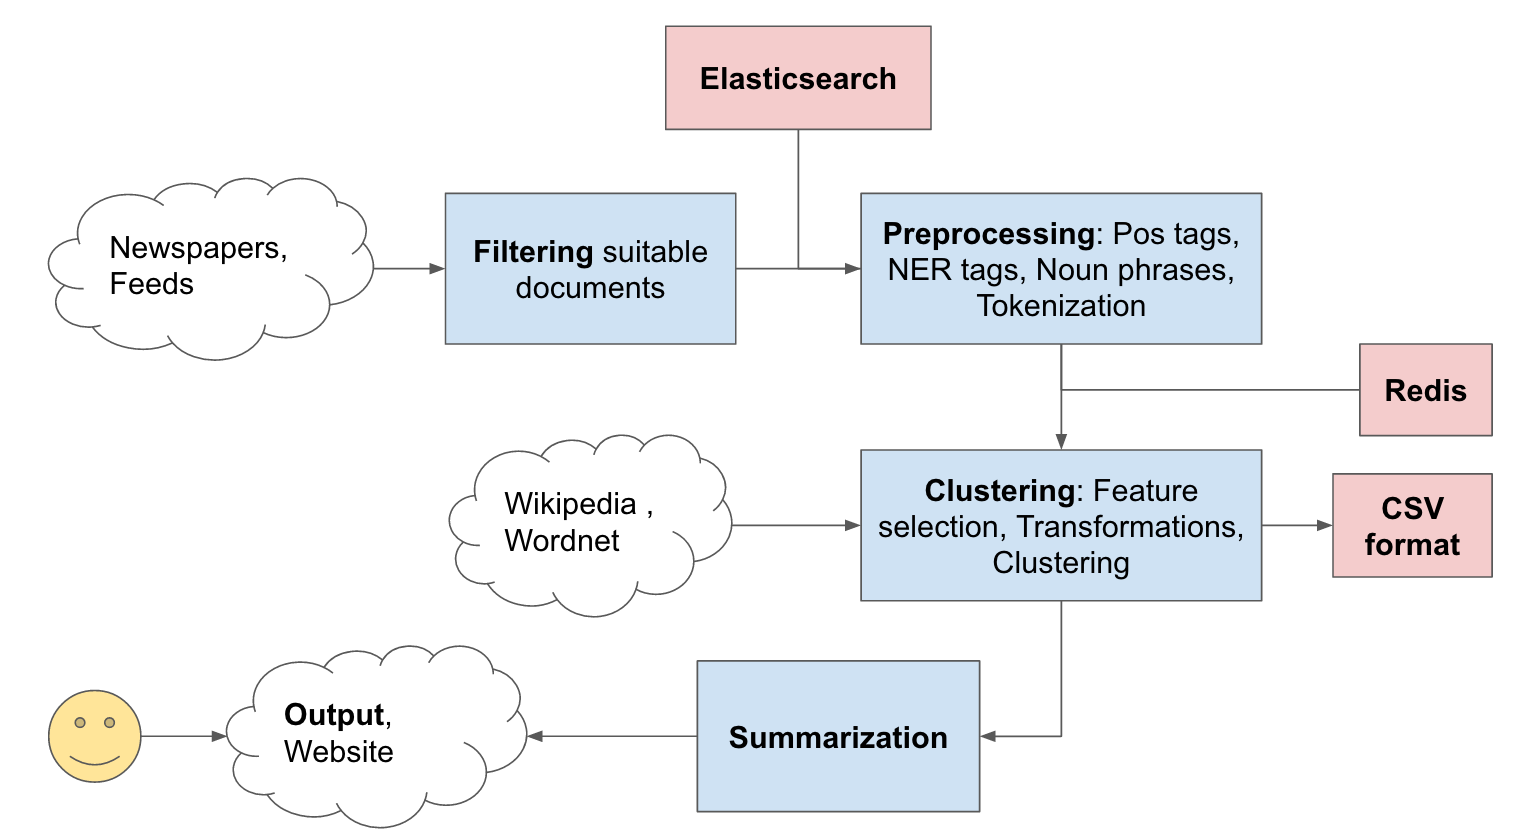
\includegraphics[width=0.7\textwidth]{news_clusty.png}
      \caption{"News-Clusty pipeline"}
      \label{news_clusty}
  \end{figure}

  The Columbia Newsblaster System by \cite{ColumbiaMultiDoc2001} is a very good point of reference. The core components of the Columbia Newsblaster are scraping, preprocessing, routing, clustering, summarizing and output generation. News-Clusty uses most of these components. They are briefly described in the following.

  \paragraph{Scraping} is the process of retrieving documents of interest in its raw form from websites, archieves and other sources. In the news domain we talk about online newspapers such as ``The Guardian'' or news feeds like google news. The inherent goal is then to persist the found pages. It is crucial to identify correct pages by several heuristics:

  \begin{enumerate}
    \item \emph{encoding} to utf-8 if working in english.
    \item \emph{language} to english, as a lot of newspapers have several languages to offer.
    \item \emph{content-length} has to be >= 500 chars to be relevant
    \item \emph{irrelevant content} like advertisement, not found pages, subscriptions etc.
  \end{enumerate}

  The more information one can collect about the article the better. Meta information like authors, meta keywords, keywords, categories, publishing dates, tags and links can be used later for more semantic strategies. Often meta keywords can completely contain what articles are about. These keywords can be reasonably used by looking up definitions on Wikipedia or Google, enhancing the content of an article. Publishing dates can be used to capture freshness by penalizing articles that are several days old.

  \paragraph{Preprocessing} is the step where raw content is send into a pipeline of filters until all noise and unnecessary information is stripped. In News-Clusty everything is on the internet in form of html pages. So a major task is to extract raw content from html to representative forms.\\
  In figure \ref{preprocessing} we work on two elastic search indices. The preprocessing module reads articles from the ``articles'' index, a continuous stream of documents and posts on the ``prep'' index. In the preprocessing we take all the actions listed and save the intermediate result as its own field. This is helpful later when computing expensive operations such as named-entity tags, noun-phrases or pos-tags. After processing the html we take a second filter step to make sure that the conditions of the scraping steps still hold true. If not the article is removed. Stripping html is not the only necessary step, we need to clean documents from bad characters, unuseful information we cannot work with like images. If the need arises spelling correction can be applied as well that is if there is sufficient evidence that articles have a lot gross misspellings, due to the central limit theorem this can be mitigated.

    \begin{figure}[h!]
      \centering
        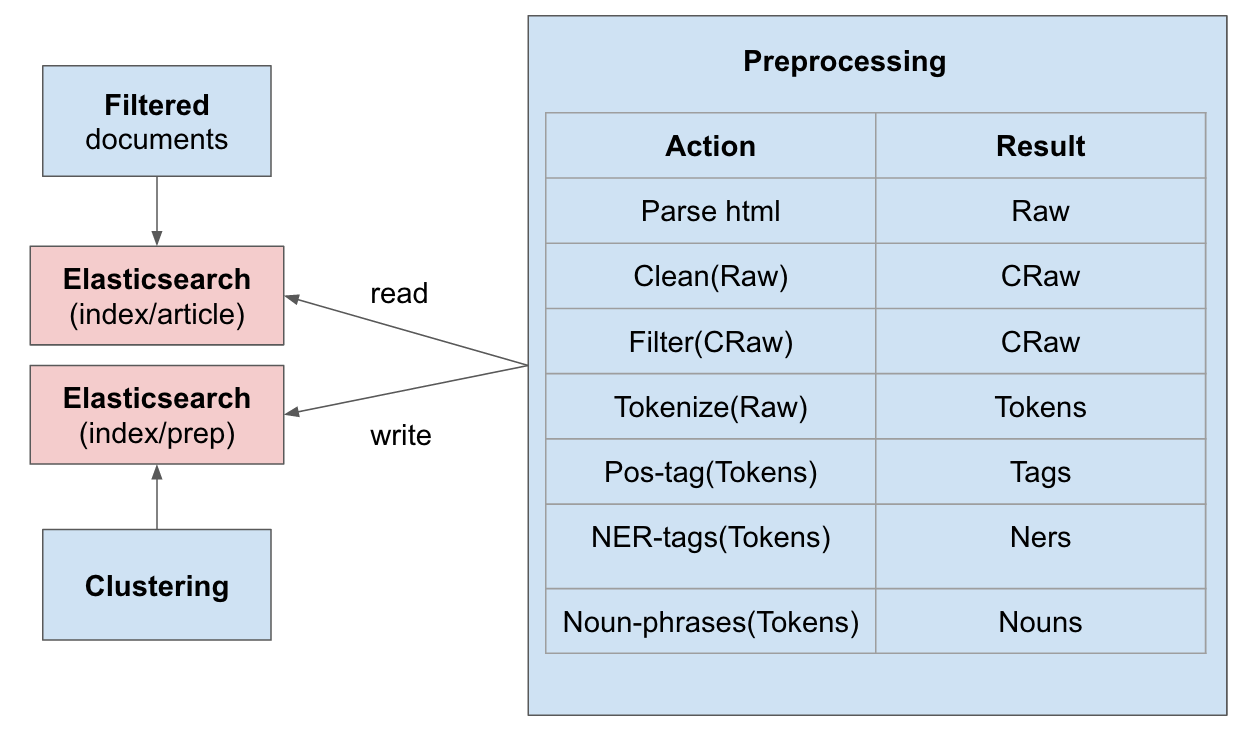
\includegraphics[width=0.7\textwidth]{preprocessing.png}
        \caption{"Preprocessing"}
        \label{preprocessing}
    \end{figure} 

  In figure \ref{preprocessing} ``Raw'' is the parsed text from the html, while ``CRaw'' represents text that contain no numbers, stopwords, short words, punctuations and special characters. The tokenization is not a whitespace splitter, it is a fully trained statistical parser that detects sentences and boundaries, as well as sentence tokens. The same goes for noun phrase extractors, pos-taggers and ner-taggers. ``CRaw'' is used as a representation of the text, while ``Raw'' is used to generate the beforementioned concepts.

  \paragraph{The Clustering} module does several transformations as displayed in figure \ref{clustering_cycle}. Feature selection is the process of picking features that are of most interest. This often happens mathematically by \emph{TF-IDF} or by formulas describing information density of words. If desired, resulting features can be enhanced by definitions and categories of \emph{Wikipedia} or projected via \emph{Wordnet} ontologies. Second transformation to any kind of vector space model like \emph{TF-IDF}, then decomposing the matrix by topic models and dimensionality reduction techniques. Before the actual clustering algorithm is run similarity matrices and normalization to unit vectors is done. After this documents can be clustered by any kind of clustering algorithm. Outcomes are evaluated and redone if desired evaluation criterias were not met.

    \begin{figure}[h!]
      \centering
        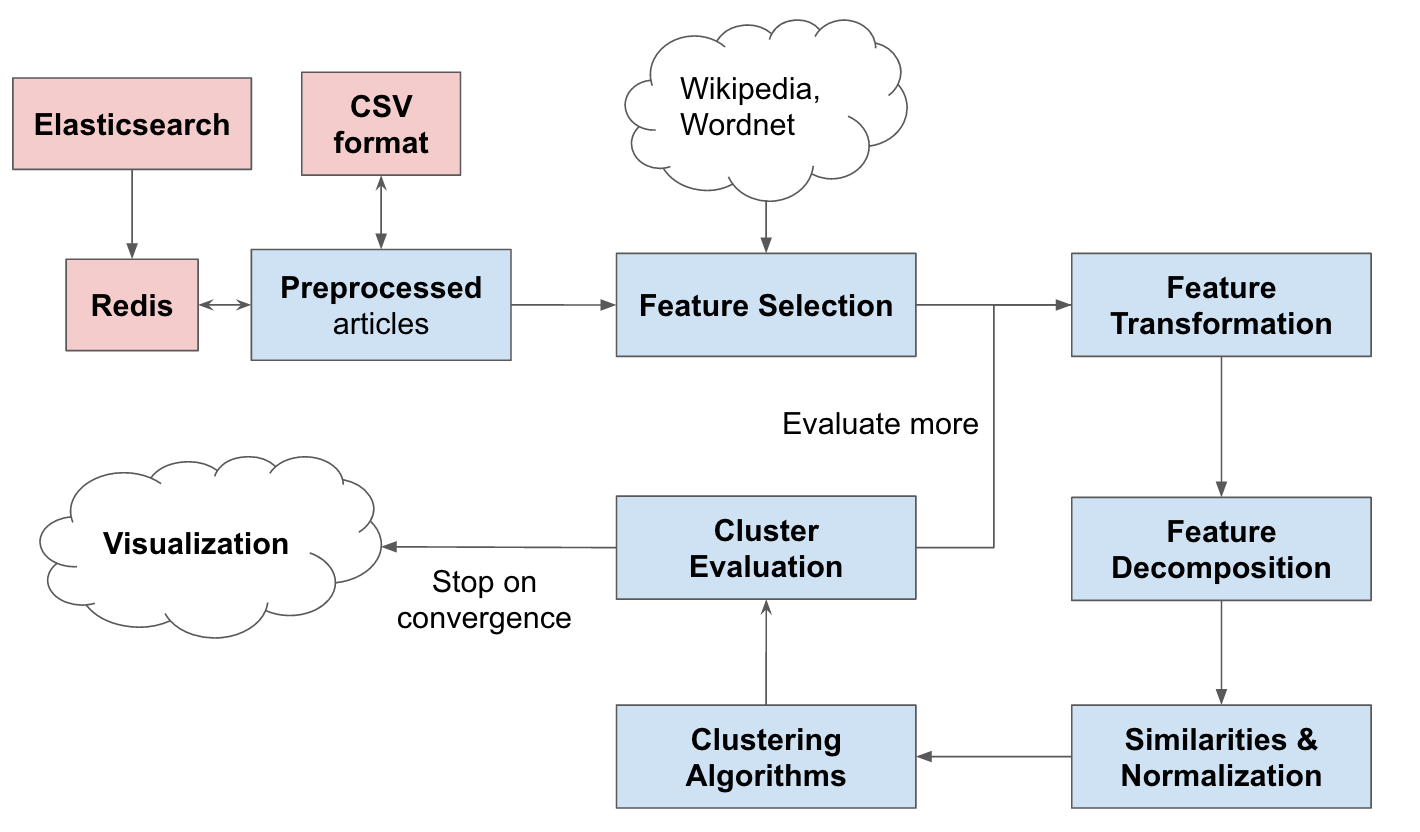
\includegraphics[width=0.7\textwidth]{clustering_cycle.png}
        \caption{"Clustering cycle"}
        \label{clustering_cycle}
    \end{figure} 

  \paragraph{The Summarization} module would receive the clustered documents as input. In addition meta information can be used here as well. The summarizer either gets single documents or a collection of documents that where in the same cluster. If assignments are soft, possible cluster overlaps can be taken into account. As this is not further part of the thesis we will leave it at that.

  \paragraph{Output generation} is a matter of visualizing the results of a summarization engine. For instance a website with rendered html. Currently clustering results can be projected to lower dimensions and to render 2D or 3D visualizations. Additionally the measures of clusterings can be compared and examined.

  \paragraph{The Routing engine} detects if the input is a type of event. They are categorized into ``single-events'', ``multi-events'', ``person-centered'' and ``other''. A single event is about the same topic e.g. the earthquake in Nepal 2015. Multi-events take place at different times, locations and with different subjects but with the same content, like terrorist attacks in 5 countries. A person-centered view is often a biography like a profile of Barack Obama running for president. This view makes it possible to make different assumptions about how articles should be summarized in case of the category of events that occured. A router like this could bring in various performance gains and strengthen the quality of a summarization. Due to time constraints this was left out of \emph{News-Clusty}.

\section{Python and Libraries}
  \emph{News-Clusty} is entirely written in the programming language Python and a well versed collection of libraries.

  \paragraph{Python} is a dynamic, object oriented higher level programming language with a rich environment for scientific computing. Python incorporates many different styles and assumptions, leading to a variety of programming paradigms between object oriented and functional programming. From the Zen of Python: ``Beautiful is better than ugly. Explicit is better than implicit. Simple is better than complex.''. For a proper introduction to Python see \cite{NltkPython}.

  \paragraph{The Persistence} of articles is held in \emph{Elasticsearch}. \emph{Elasticsearch} is a document store that can be easily distributed accross hundreds of nodes. It is schemaless and can be dynamically adjusted if need be. Its primary use case is for search and anything related to huge chunks of text. \emph{Redis} on the other hand is used as a cache for different feature selection strategies. It is a key value store and commonly chosen for fast execution. The common strategy is to first generate feature sets by querying \emph{Elasticsearch}. Each successful feature selection on a document will be persisted as a numerical feature vector into \emph{Redis}. Multiple accesses to the same documents will be read from \emph{Redis} if possible.\\
  While databases have huge advantages by querying documents, there is an overhead when accessing all files at once. If for a particular reason a whole dataset must be used, it is advised to use some of the serialization tools that output sparse matrix market formats or serializes to raw text files. Input and output on filesystems is faster if you do not need to query the data. This holds true as long as a single node filesystem is involved. \emph{Elasticsearch} for instance has its powers by leveraging clusters of servers (nodes).\\ 
  The indices for \emph{Elasticsearch} are scoped by the scraping date, $20150701/article/id = document$ or $20150701/prep/id = document$. This is particulary helpful if continuous processing, day by day, is an objective. The reason for choosing both is that we get highly expressive power and fast solutions for document queries and caching. If for several reasons the system should be setup in a distributed system of server nodes, both databases come with well defined abstractions.

  \paragraph{The Libraries} used throughout \emph{News-Clusty} are well-versed scientific data processing libraries. The library creators and maintainers should be mentioned and accredited for. \emph{News-Clusty} leverages linear algebra, feature selection strategies and clustering algorithms from \emph{Scipy} (especially numpy and sklearn) see \cite{ScikitLearn}. It uses natural language analysis tools from the nltk by \cite{NltkPython}. Moreover named entitiy recognition by the \emph{StanfordNLP group}, noun phrase extraction by \emph{Conll}, word ontologies by \emph{Wordnet}, knowledge and dictionaries by \emph{Wikipedia}. Additionally \emph{newspaper3k} for scraping newspaper articles and \emph{gensim} build by \cite{gensim2010} as high level abstractions for probabilistic topic models. In the future it would be good to rely less on certain libraries where it makes sense, e.g. not using \emph{newspaper3k} for scraping or \emph{Scipy} for clustering algorithms.




      

    \chapter{Feature Selection}
      \label{chapter:feature_selection}
      \epigraph{\emph{
  ``Coming up with features is difficult, time-consuming, requires expert knowledge. "Applied machine learning" is basically feature engineering.''
}}{ Andrew Ng }

Considering the ``right'' features for clustering is a demanding and error prone process. Currently there is really just one way of describing documents: The vector space model. It breaks down to counting occurences and cooccurences of words and measuring distance by mathematical functions. We could just take all the words of a document, removing stopwords, and put them into a feature vector. This results in dimensionality explosion and extreme noise. Contrary to a document vector $d = \{w_1,w_2..w_n\}$, the feature vector represents a document by concepts $\{c_1,c_2,..c_j\}$. It is a projection of the original document $d = \{w_1,w_2..w_n\}$ to more general concepts resulting in fewer dimensions. This lifting is bestly described as combining several words of a document, often occuring in the same sentence, extracting a shared meaning. We hope to find fewer words that share enough information with the original word, that the following holds:
  
  \begin{equation}
    f : d=\{w_1,w_2,..w_n\} \to \{c_1,c_2,..c_j\}
  \end{equation}

The function $f$ transforms a sequence of words $w_1..w_n$ of a document $d$ to a sequence of concepts $c_1..c_j$. The concepts can be derived in a lot of ways.

  \begin{enumerate}
    \item Pruning words of low and high significance.
    \item Using syntactic parsing to retrieve noun phrases, named entity tags or part of speech tags.
    \item Using ontologies of \wordnet{} to derive a shared meaning of words.
    \item Mapping documents to \wiki{} categories.
    \item Using kernel methods, preselecting initial clusters in a semi-supervised way.
  \end{enumerate}

In the end, feature selection is probably the most demanding task. Expert knolwedge needs to be applied and can change over time, called time drift. A computer handles documents in vector space, by counting. A human however perceives content differently. For any sufficiently adavanced algorithm that works with a knowledge base it is still: Garbage in, garbage out. More fancy algorithms will lead to better results, but better features will accelerate the accuracy.\\

In the following we will briefly explain what \emph{semantics} mean, especially in the \emph{domain} of newspapers. How \emph{feature selection} generally works and how this can be enhanced by \emph{syntactic parsing}. Strategies using \wordwiki{} are explained. In the experimental chapter we will then present how all these mechanisms come together.


\section{Semantics}
\label{sec:semantics}
  
  Semantics is the study of meaning. Given some symbols, characters, words or phrases what is their underlying meaning? The question is inherently hard and lots of literature focuses on how computers can get better at this. Most of the concepts depicted here taken from \cite{NLPBookJurafsky2000}. Semantics can also be viewed from a statistical point of view. Given a lot of phrases and words, can we infer their underlying structure that generated them? How can statistical patterns reveal what was meant and to what degree?\\
  In computational linguistics we often speak of \emph{word-sense disambiguation (WSD)}. \emph{WSD} is short for identifying sense of a word, if a word can have several meanings, in a sentence or paragraph. The sentence\\ 

    \emph{``The bail out during the financial crisis of the Lehmann brothers bank, was much too late.''}\\

  makes it obvious that it is about financial institutions ``bank'' during the financial crisis, political intervention by providing money ``bail out'' and a specific financial institution or entity ``Lehmann brothers''. How could we possibliy discern such a sentence so that we can actually reveal all the beforementioned concepts? To successfully find such concepts we have to identify what parts of speech, e.g. nouns, verbs, adjectives etc., each word of a document has:

    \begin{equation}
      pos\-tag(d=[w_1,w_2,..w_n]) = [(w_1, tag_1), (w_2, tag_2),.. (w_n, tag_n)]
    \end{equation}

  Part of speech tagging works by parsing a document sentence by sentence. Tagging each word by identifying its position relative to other words and predicting what their tags might look like. See \cite[chp. 5]{NLPBookJurafsky2000} for an extensive study.
  For clustering we want to identify these \emph{semantic fields}, a set of words grouped by meaning. We then often analyze \emph{WSD} through \emph{synonymy, polysemy, hyponymy, hypernymy and meronymy}. All of those concepts are important to taxonomies and ontologies. A \emph{taxonomy} is refered to as a simple hierarchical structure of parent-child relationships, that change in granularity per hierarchy level. An \emph{ontology} is much broader and can have complex relations other than parent-child. In that sense both taxonomies and ontologies are structures, showing how to classify words in context to each other. Traversing through these hierarchical structures is typically done by hyponyms and hypernyms. 

    \begin{figure}[h!]
      \centering
        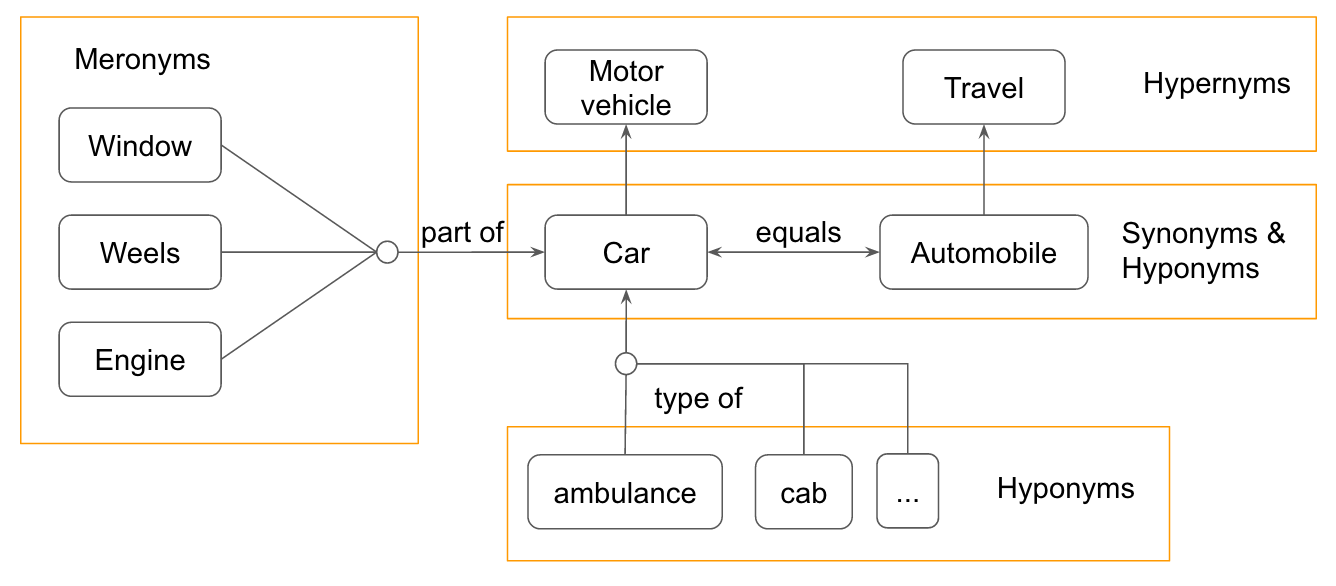
\includegraphics[width=0.9\textwidth]{wsd_analysis.png}
        \caption{"Semantic fields, hierarchies"}
        \label{wsd_analysis}
    \end{figure} 

  \emph{Meronyms} are ``part-of'' relations, \emph{hyponyms} have a ``type-of'' relation to a higher concept, called \emph{hypernyms}. In figure \ref{wsd_analysis} we see that from a single concept ``car'' we can infer a semantic field around it. We will see later how this works, a statistical concept around this is \emph{LSI} and \emph{probabilistic topic modelling}. The symbolic way is to use knowledge bases such as \wordwiki{}.\\

  In the text \emph{domain} of newspaper articles a few problems arise. Analyzing a long book, a long speech or journal articles from the scientific community, is easier compared to high varying fragments from different authors on different topics. A long book written by one person will use a specific language that is typical of that author. Speeches for a specific person contain similar concepts and often use the same language as well. In the scientific community rhethorial and anecdotal phrasing is uncommon. Facts, citation and correct formatting is of central importance. The text might be heterogenous but the fact remains that a certain wording / glossary, is shared throughout these examples.\\

  This does not hold true for newspaper articles. \emph{Topics} about different events co-occuring on the world. Different \emph{authors} with different writing styles. Different \emph{newspapers} with different directions of content presentation. \emph{Long} and very \emph{short} articles. And this does not take images, videos or comments into account. When dealing with a vast landscape of different topics, spanning connections between two documents becomes a hard task. In context of such sparse data, that is documents with almost no connecting words, clustering works poorly. This can also be described as a high variance problem, where each document contributes a lot of unseen words to the feature vector.\\

  In order to avoid these variance problems, we need to find a solution to \emph{WSD} and then apply a lifting from the original concept to a hypernym. Going back to figure \ref{wsd_analysis} we see that \emph{car} and \emph{motored vehicle} might mean the same thing. Both are about cars, if we project the concept \emph{car} to \emph{motored vehicle} the concept would connect both the documents containing car and motored vehicle. This is not always what we want to achieve but it could drastically improve similarity between documents that would miss each other by synonymy and polysemy.

\section{Selection}
\label{sec:selection}

  As described before we want to tackle \emph{WSD} and find ways to connect documents that share common meaning but not a lot of common words. To do so we have several strategies at our disposal. First, word pruning is presented, it is probably the most widely used technique for lowering dimensions and removing insignificant words. Second, synctactic parsing is described in by part of speech tagging, noun phrase extraction and named entity recognition. One topic which is left out are the kernels. They are important to retrieve better results in a semi supervised way but could not make it into the thesis experiments.

  \subsection{Word pruning}
  \label{sec:word_pruning}

    Before pruning words we have to convert the documents into a suitable vsm such as \emph{counting vectors} or \emph{TF-IDF} described in \ref{sec:bag_of_words}. The counting alone in its basic form is sufficient in telling if a term has a high or low connection with all other documents. The \emph{TF-IDF} on the other hand is a measure of importance and solely based on the resulting frequencey per word. It is possible to make significant pruning on both representations. The \emph{TF-IDF} variant is prefered as it normalizes frequencies. Higher or lower counts are weighted into a formula that better represents the significance of a term.\\

    Either way we need to create a cooccurence matrix $M = count(C, D)$ where $C$ is a corpus and $D$ is the dictionary of the corpus. Then we transform by $M = tfidf(M)$ or leave it with the \emph{term frequency}.\\

    Pruning $M$ is done by cutting off the documents with a very low ratio of counts with respect to all documents. This can be done by threshold in proportion to all terms, a percentage, removing $j$ terms. It can also be achieved by a hard count, cutting of all terms that have no counts higher than that. This means, we remove insignificant terms or terms that do not contribute to any connection. Semantically this means, we cut off words that have a high meaning in a single document and a very low in others. Those words are redundant, or in other words they have no discriminant value to the clustering process.

      \begin{equation}
      \begin{split}
        m &= [0, 1, 5, 0, 4, 0, 1, 1, 2, 3] \\
        m_s &= sort( [0, 0, 0, 1, 1, 1, 2, 3, 4, 5] ) \\
        percentcut(m_s, 0.2) &= [0, 1, 1, 1, 2, 3, 4, 5] \\
        totalcut(m_s, 1) &= [2, 3, 4, 5]
      \end{split}
      \end{equation}

    The min cut on percentage $0.2 = 20\%$ cuts the first 2 samples or removes the first 6 in case of a total count. The parameter has to be varied, depending on the outcome of a cost function. Further we can take off the top $j$ words as well by the same principle. The problem with the top words is, that they highly correlate with a lot of different documents, meaning a high correlation between a term and the corpus. Leaving them out erases a lot of connections, resulting in more discriminant features. This is what we want to achieve, finding the middle words, that are common in certain documents and uncommon in others. During clustering this will result in much more coherent clusters.

      \begin{equation}
      \begin{split}
        m &= [0, 1, 5, 0, 4, 0, 1, 1, 2, 3] \\
        m_s &= sort( [0, 0, 0, 1, 1, 1, 2, 3, 4, 5] ) \\
        maxcut(m_s, 0.8) &= [0, 0, 0, 1, 1, 1, 2, 3]
      \end{split}
      \end{equation}

    The max cut works with a ratio that selects from lowest to highest 80\% except the last 20\%. Note that the samples are not on $m$ dimensional vectors. For this to work we have to aggregate the counts and then prune the most insignificant words. The great thing of this approach is that it can follow any feature selection strategy. By using word pruning on feature vectors, the selection process can be refined. The fine tuning is necessary in gaining percentages in accuracy.

  \subsection{Syntactic parsing}
  \label{sec:syntactic_parsing}

  Parsing reduces symbols, to a parsed tree of following expressions. In English parsing, probabilistic shift reduce parsers in combination with trained neural networks is state of the art. \cite{ShiftReduceParsingStanford} Valid words and characters are defined within the rules of the English alphabet. In figure \ref{syntactic_parsing} we can see a parse tree for an English sentence parser. The parsing is syntactical based on English grammar. When it comes to parsing expressions from English language to a meaningful representation for the computer, the problem statement gets a lot more difficult. Too many words, too many forms of sentences - statistics in combination with structural parsers come to the rescue. Solely syntactic parsers that work on symbols work well in a specific domain up to a certain parsing accuracy. Statistical models remove these barriers by likelikhoods and predictions, finding answers accross domains. The most inherent problem is overfitting. Overfitting describes that a probabilistic parser works well on a specific problem domain or data source, because it learned the domain well. Unseen domains and datasets perform poorly due to the missing knowledge. The problem becomes more clear, in the domain of newspaper articles where different language styles and domains are frequent. Statistical parsers like the \emph{Stanford} parser are very accurate in identifying valid syntactic English expressions. In the following we will look more closely at noun phrase extraction and named entity recognition. They can be used as initial seeds for the feature space of a corpus.

    \begin{figure}[h!]
      \centering
        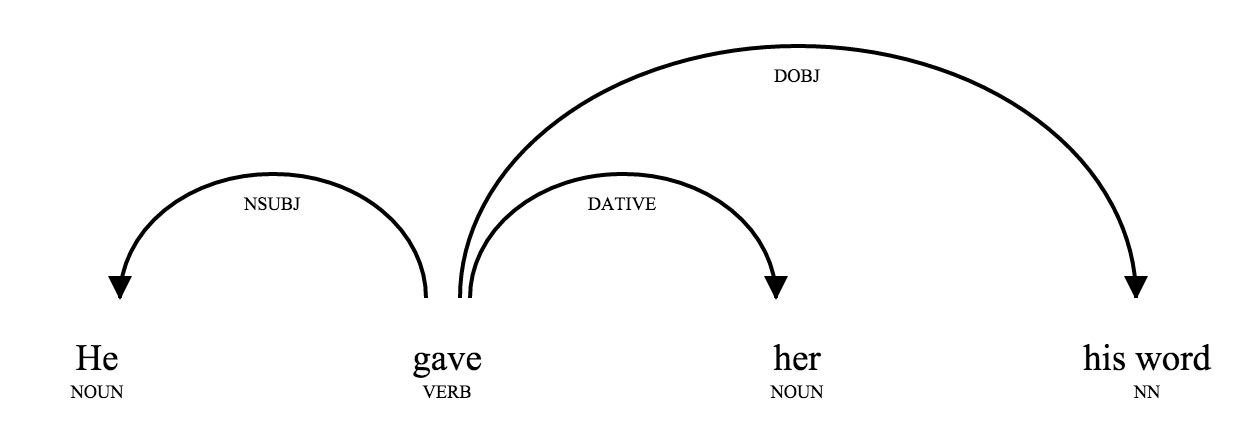
\includegraphics[width=0.9\textwidth]{sentence_structure.png}
        \caption{"Syntactic parsing"}
        \label{syntactic_parsing}
    \end{figure} 

  Figure \ref{syntactic_parsing} is displayed as a projective tree, where each word has exactly one (or none) incoming and outgoing edge. The outgoing edge is refered to as head. Edges contain information about the relation between both words. Each word has a part of speech tag described by many corpuses. Current research projects use Googles ngrams over time, with a 3 billion ngram corpus to infer the most likely structures. \cite{SyntacticNgramsOverTime2013}
  The parsing of English grammatical structures is entirely dependant upon specification of the rules. What part of speech tagging system is used? How is the grammar defined? With the help of the Chomsky hierarchy it was proven that not all natural languages have context-sensitive (type-1) nor turing complete (type-0) grammars. See \cite[chp. 16]{NLPBookJurafsky2000} for a great introduction.
  In clustering this is not a huge problem, because the granularity of the task is not that fine tuned. A slightly false parse might still yield good feature results.

  \subsubsection{Noun phrases}
  Noun phrases are often referred to as key phrases. Formally a noun phrase is a phrase with a noun as its head word. A head is a word that determines the syntactic type of a phrase. Generally a noun phrase is a part of a sentence that captures meaning of a sentence. Thusly they are good samples to represent a document. However noun phrases are rather bad samples for clustering. They do not connect well to other documents due to their unique occurences. In the \wordnet{} section we will see how they are great for projecting to their respective hypernyms. Noun phrase extraction is highly connected with part of speech tagging where certain tag patterns are used to filter nouns or noun phrases. For further information see \cite[chp. 5, 12]{NLPBookJurafsky2000}.

  \subsubsection{Named entities}
  Named entity recognition is the task of information retrieval that extracts and classifies  names of persons, organizations, locations, expressions of times, quantities, monetary values, percentages, etc. \cite[chp. 22]{NLPBookJurafsky2000}. 

    \begin{figure}[h!]
      \centering
        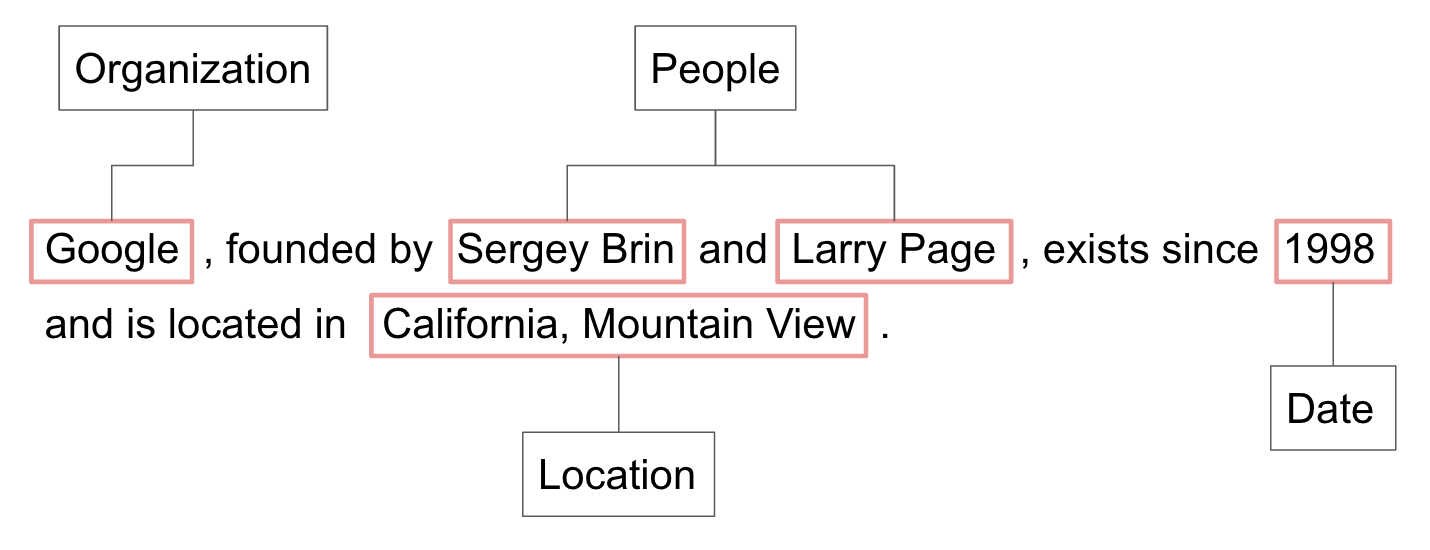
\includegraphics[width=0.9\textwidth]{ner_tags.png}
        \caption{"Named entities"}
        \label{ner_tags}
    \end{figure} 

  As seen in figure \ref{ner_tags} we are interested in informative terms. Often occuring named entities tend to give a direction what a document is about. If Google occurs in one document, it most likely will have to do with a lot of other documents that are about Google. We would like to favor documents that are connected by their respective named entities and weight them in more than others. Named entities like noun phrases are very discriminative. In systems like the Columbia Newsblaster system, named entities would be used to determine if a document is rather biographical or has todo with an event of the past. \cite{ColumbiaMultiDoc2001}

\section{External Knowledge}
\label{sec:semantic_selection}

  In order to enhance the syntactical selection models we can add a knowledge base such as \wordwiki{}. The data reresentation is often defined as a typical dictionary. For a definition of a word we can infer semantic fields and additional text describing the words in more detail. Moreover knowledge bases such as \wiki{} categorize/classify concepts into ontologies. \wordwiki{} are great in the sense that human authors around the world add missing information and enhance the models frequently. The knowledge bases are enhanced frequently by writing rules and reviewing processes.

  \subsection{WordNet}
  \label{sec:wordnet}

  \wordnet{} is a lexical database of English. Lexical parts of speech such as nouns, verbs or adjectives are grouped into synonyms (synsets). Each synset is linked by semantical and lexical relations. In parts \wordnet{} resembles a thesaurus, grouping words based on meaning. With its onotologies it deals with \emph{WSD}. Further words are interlinked by semantic relations. For more information see \cite{Wordnet1995, Wordnet1998}. \\
  \wordnet{} is often used for lemmatization. Lemmatization is the process of removing the inflected forms of a given word to its lemma. A lemma is a dictionary entry or canonical form of a word. The major difference to stemming is that \wordnet{} is able to inflect a canonical form that depends on context sensitive pos tags. 

    \begin{equation}
    \begin{split}
      lemmatize("savings", pos="noun") &\to "saving" \\
      lemmatize("savings", pos="verb") &\to "save" \\
      stem("savings") &\to "save" \\
      stem("save") &\to "save"
    \end{split}
    \end{equation}

  Inflecting the canonical form with pos tags enhances the precision of the context where the words came from. Often this can result in different inflectional forms that would otherwise be equal. In comparisson we can see that stemming treats ``savings'' and ``save'' entirely the same. This is a basic strategy to inflect a generalized version of a document, to lower the dimensions. Further we can take the hypernyms of a document.

    \begin{equation}
    \begin{split}
      \sum_{i=1}^{|d|} hypernyms_{first}(d_i)
    \end{split}
    \end{equation}

  We iterate over all words in $d$ and take the first of the hypernyms of the words, projecting it to a higher concept. \wordnet{} sorts the hypernyms from most likely to less likely, taking the first is a good approximation.
  Enhancing the above statement we scale this up to the depth $d$ going up the hypernyms of the \wordnet{} ontologies.

    \begin{equation}
    \begin{split}
      closure(seq, d=0) &= empty \\
      closure(seq, d>0) &= \sum_{w \in seq} closure(hypernyms(w), d-1)
    \end{split}
    \end{equation}

  At last, we can infer the most common meaning of a sentence by calculating the lowest common hypernyms. 

    \begin{equation}
      lowest\_common\_hypernyms(w_1, w_2) = hypernyms(w_1) \cap hypernyms(w_2)
    \end{equation}

  For this we compute for each word in a document the transitive closure with the above statement not restricted by the first hypernym.

    \begin{algorithm}[H]
    \begin{algorithmic}[1]
      \caption{\wordnet{} closure with hypernyms}\label{wordnet}
      \For{$sent \in closure(doc, d)$}
        \For{$(w_1, w_2) \in sent : w_1 \not = w_2$}
          \State $result \gets lowest\_common\_hypernyms(w_1, w_2)$
        \EndFor
      \EndFor
      \State \Return $result$
    \end{algorithmic}
    \end{algorithm}

  Then we compute the lowest common hypernyms that connect hypernyms of the word closures. We then apply word pruning to get the mid vector words, sorting out extremes. It is also possible to greatly enhance the above models with lexical chains, see \cite{SemanticClusteringWithWordnet} for more.

  \subsection{Wikipedia}
  \label{sec:wikpedia}
    




    \chapter{Clustering experiments}
      \label{chapter:clustering_experiments}
      \epigraph{\emph{
  ``An algorithm must be seen to be believed.''
}}{ Donald Knuth }

In this section we evaluate some strategies for clustering. At first we will show how a single day of news events are clustered. Then clustering news events over multiple days. Due to time constraints it was not possible to elaborately test multiple days clustering. It is a notoriously difficult topic that greatly relies on the data and time. Originally it was intended to use a scraped data set over several month, categorized by date, with as much meta data as possible. As this is at the barrier of legality, a smaller standardized data set namely the BBC data set by \cite{BBCData2006} was used. In the original data set it was possible to assume that the data was ordered and sorted by day. Several thousand articles could then be easily clustered on a daily basis and enhanced over the course of several months. Instead we are focusing on how the BBC data set can be clustered and evaluated. Multiple day clustering will be depicted, but not in any form evaluated.\\

The BBC data set had a few limitations in the sense that dates were not provided and meta data not provided by the authors. As such we treat the data as a a bulk of events occurring in the time frame of 2004-2005. Fortunately unlike real world data the articles are tagged with precise categorical labels, so external evaluation measures were an option. There were limitations in time to find a more adequate set of articles that were consecutively sorted by day in a broader category such as ``world news''.\\

The clustering was done in several steps, similar to the Columbia Newsblaster system.\cite{NewsBlaster2002} A hierarchical clustering approach by first clustering events into categories like politics, business or entertainment and second clustering the categories into distinct events. The classification in the first step guarantees some broader topical cohesion. In the BBC data set a purity of up to 94\% could be achieved on the test set. This is unusually high, but is probably due to the normalized data set that represents the classes exceptionally well. The real world data set could go as high as 45\% purity and less. The purity on the BBC data set varies broadly between 79\% and 94\%. This variability results in overlapping topics where the majority of documents in a cluster are in the same class. Each of the resulting clusters resembling the underlying classes are re clustered. A clustering algorithm that optionally does not take any constraints on the amount of clusters is used. In this second step clusters represent news events on several topics per cluster.\\

Some final words on the measurement of the two steps. In the first step it is easy to evaluate how well documents were assigned to their respective classes. In the second step however evaluation is not that simple. At this point, we are interested in document similarity based on content and not class labels. The results of the second clustering are informal and not measured.

\section{Single day clustering}

Single day clustering is done by focusing on one specific date. The hypothesis is, as long as there are no major news headlines, documents will have a high variance in vector space. Thus there will be more clusters. The major news headlines is important, because, during the original data set scraping there were ground breaking events, that literally absorbed almost all articles into single clusters. That was expected because roughly 90\% of the articles were about the same news event. The angle of the different articles covering the event varied greatly enough that topics that had no underlying connection to the event were clustered into as well.\\

In the following the two steps are refined. First we want to classify news events by classes, in case of the BBC data set: politics, business, entertainment, tech and sports. For this it is possible to use algorithms with a hard number of final clusters to classify documents into the classes. Alternatively one could use a supervised classifier, which in practice, is much more accurate. See \cite{LearningMultiLabelKmeans2013} for a real world example learning labels in comparison of \emph{K-Means} and a \emph{supervised classifier}. Second the resulting clusters, now assigned by news category are clustered again. This time the clustering algorithm has the constraint of automatically detecting the cluster numbers. For this a hierarchical algorithm with soft thresholds was chosen like BIRCH or Ward linkage. The resulting clusters resemble news events dealing with a similar topic. 

\section{Implementation}
The implementation of a more general clustering algorithm in the text domain can vary drastically. A general scheme is given by algorithm \ref{general_clustering}.

  \begin{algorithm}[H]
  \begin{algorithmic}[1]
    \caption{General clustering}\label{general_clustering}
    \Function{general\_cluster}{$X_{train},y_{train},\kappa,\alpha,d$}
      \State $X_{norm},y_{norm} = normalize_{text}(X_{train},y_{train})$
      \State $X_{project},y_{project} = project(X_{norm},y_{norm})$
      \State $X_{trans},y_{trans} = transform(X_{project},y_{project})$

      \State $X_{lsi} = lsa(X_{trans}, topics=\alpha)$
      \State $X_{dim} = reduce\_dimensions(X_{lsi}, dimensions=d)$
      \State $X_{sim} = similarity(X_{dim})$
      \State $X_{scaled} = scale(X_{sim})$
      \State $model,centroids,labels,k = cluster(X_{scaled}, clusters=\kappa)$

      \State \Return $model,centroids,labels,k$
    \EndFunction
  \end{algorithmic}
  \end{algorithm}

The general implementation \ref{general_clustering} is separated into several steps. As input the function gets a training set $X_{train}$ and a label set $y_{train}$. $\kappa$ is an optional parameter for the total amount of cluster centers. $\alpha$ a parameter that sets a desired size of topics for models like \lsa{}. And a dimension $d$ to reduce $X$ to for visualization purposes by e.g. \pca{}. In general we assume that the data $X_{train}$ is of any textual sort, the preprocessing needs to do the necessary steps that fits the function. Moreover it is of utmost importance to think in terms of vectorized code. Any procedures gradually transform a document into the vector space. After this all rules by linear algebra hold.

  \begin{enumerate}
    \item \emph{normalize} takes $X_{train}$ and $y_{train}$ to remove special characters, stop words, numbers. Lower casing any words and removing non English characters or sentences. 
    \item \emph{project} is any kind of projection strategy via \wordnet{}, noun phrases or named entities, lowering word sense disambiguation and dimensions. This step deals with the initial seed of knowledge that is used throughout the algorithm.
    \item \emph{transform} takes in the projected data and transforms it via TF-IDF, word pruning, as well as ngram enhancement.
    \item \emph{lsa} is an optional step that transforms the resulting data to dense low dimensional matrices, keeping as much variance as possible while reducing noise. In this case \lsa{} was used but \lda{} or \hdp{} would be an option as well. 
    \item \emph{reduce\_dimensions} is an alternative step that reduces the dimension of the data to 2d or 3d plotting clusters. This is typically done by \pca{}.
    \item \emph{similarity} transforms document x term vectors to document to document similarity by cosine or euclidean distance measures.
    \item \emph{scale} is a second normalization step, scaling the data by variance and average.
    \item \emph{cluster} finally takes the matrix $X_{scaled}$ and clusters based on a hard constrained clustering number. If not supplied the clustering algorithm needs to predict a cluster number automatically. This results in the actual cluster amount $k$. The resulting trained clustering $model$. The $centroids$ in case they are actively calculated e.g. by \emph{K-Means}. And finally the $labels$, the assignment from a document to a corresponding cluster.
  \end{enumerate}

The implementation is a rough sketch of a real clustering scheme. In reality most of the before mentioned steps can be parameterized or constrained by additional arguments. Either a configuration object is specified or an extensive API used to create clustering scripts. The API used was $scikit-learn$ by \cite{ScikitLearn} and is part of the huge scientific computing libraries written in Python, such as $numpy$, $scipy$, $pandas$ etc. From this we can generalize for a clustering scheme over a single day.

  \begin{algorithm}[H]
  \begin{algorithmic}[1]
    \caption{Single day clustering}\label{single_day_clustering}
      \State $X_{train},y_{train} = get\_data(timestamp)$
      \State $model,centroids,labels,k = general\_cluster(X_{train},y_{train},\kappa,\alpha)$
      \State $X_{assigned} = get\_assigned\_documents(X_{train},labels)$
      \State $news\_labels = []$
      \For{$c \in X_{assigned}$}
        \State $model',centroids',labels',k' = general\_cluster(c,nil,\alpha)$
        \State $assign(news\_labels, X_{train}, labels')$
      \EndFor
      \State \Return $news\_labels$
  \end{algorithmic}
  \end{algorithm}

The implementation \ref{single_day_clustering} is a rough sketch of what the \emph{News-Clusty} system does. First get the data by a timestamp e.g. ``20150701'', cluster the data by a fixed $\kappa$ and then use the resulting cluster assignments $X_{assigned}$ to group news events. Note that $general\_cluster$ in the second run has a $nil$ argument, because we do not want to constrain by cluster amount. The clustering now depends entirely on the variation of the intermediate procedures of $general\_cluster$ and is now an optimization problem. 

\section{Evaluation}
In the evaluation section the before mentioned measuring strategies are used. Several different strategies are weighted against each other. It was found, that there are several different ways with a good performance in the categorical clustering approach. The second clustering is not of utmost importance in the evaluation but is depicted later on. A major problem is, that several parts of the proposed algorithm has parameters that need to be estimated. To narrow down this combinatoric explosion of parameters, several assumptions can be made.

  \begin{enumerate}
    \item Limiting the strategies to simple word tokens and their document titles except stop words, noun phrases and NER tags as well as \wordnet{} first hypernym and \wordnet{}lemmatization.

    \item \emph{Transforming} by \emph{TF-IDF} with a 80\% maximum threshold and a hard count $3$ for minimum threshold, excluding ngrams.

    \item \emph{topic modeling}, whether \lsa{} or \lda{} should be used or not. The topic size is manually adjusted.

    \item Setting the \emph{distance measure} to \emph{cosine}.

    \item \emph{clustering algorithm} constrains, such as density thresholds and maximum \emph{HAC} depths. Classification is constrained by $k=5$ for the categories of the BBC data set.
  \end{enumerate}

A comparison of the different strategies with \lsa{} enabled, for the classification task, is shown in table \ref{comparison_single_with_lsa}. Note that the \emph{purity}, \emph{v-measure} and \emph{silhouette score} is averaged over 5 consecutive runs.

  \begin{table}\label{comparison_single_with_lsa}
    \begin{tabular}{ c | c | c | c }
      Strategy    & v-measure & purity  & silhouette \\ \hline
      Word tokens & 0.812     & 0.926   & 0.118      \\
      Syntactic   & 0.795     & 0.916     & 0.109 \\
      Word + noun tokens & 0.826   & 0.934     & 0.118 \\
      \wordnet{} $hypernyms_{first}$ & 0.710   & 0.884     & 0.068 \\
      \wordnet{} lemmatization   & 0.726   & 0.895     & 0.069 \\
    \end{tabular}
    \caption{Comparison of feature selection with \lsa{}}
  \end{table}

Concluding from this, word tokens in combination with noun phrases lead to the highest v-measure. While other strategies perform still well enough, the chance for the best classification by clustering stems from purely syntactic means, e.g. word tokens and noun phrases. With \wordnet{} lemmatization we have a highly effective approach. That is, from the original 12000 feature dimensions we projected to 6000. Except for lemmatization, \wordnet{} approaches performed worse than the mentioned strategies. This is not generally the case as can be seen in \cite{TopicClassificationReuters2002} for an example on the Reuters Corpus with \wordnet{} using a multinomial Naive-Bayes classifier.\\
We can see in table \ref{comparison_single_without_lsa}, that the same measurement without \lsa{} performs in almost all instances worse. Note that \lda{} was explicitly excluded from the possible topic modeling techniques as it promotes a poor pre clustering step. This is due to the fact that \lda{} maps several topics to documents, resulting in documents having assignments to many topics. This is a desired property for the second clustering run.

  \begin{table}\label{comparison_single_without_lsa}
    \begin{tabular}{ c | c | c | c }
      Strategy    & v-measure & purity  & silhouette \\ \hline
      Word tokens & 0.667     & 0.831   & 0.073      \\
      Syntactic   & 0.634     & 0.794     & 0.067 \\
      Word + noun tokens & 0.666   & 0.831     & 0.074 \\
      \wordnet{} $hypernyms_{first}$ & 0.585   & 0.784     & 0.048 \\
      \wordnet{} lemmatization   & 0.585   & 0.784     & 0.048 \\
    \end{tabular}
    \caption{Comparison of feature selection without \lsa{}}
  \end{table}

The discrepancy between v-measure, purity and silhouette is expected. v-measure takes into account that several clusters contain an amount of labels that are not dominant. The higher the variance of spreading labels, even if their occurrence count is low, leads to a penalty in v-measure. Purity on the other hand compares how many dominant labels are in one cluster and penalizes for each non dominant label. It does not account for the variety of falsely assigned labels. The silhouette score is extraordinary low due to the high dimensionality. It can not be taken in absolutes but rather in relative terms between different strategies. The higher the score the higher the cohesion between topic segments. In total, the silhouette score is better when the purity and v-measure is relatively higher.

\section{Experimental}
While clustering for classification is a very good first step to pre select documents into isolated clusters, the requirements change in the second run. The results do not need to be constrained by cluster amount. Selection of similar news events return smaller topical clusters. It is difficult to show that a connection between different documents can be made when no information about time are present. If a document about ``taxes in the us'' occurred at a specific day and a second document about ``Obama raises taxes'' at the next day occurred, we could conclude that it is a current topic in the news that are related. Without knowing when a document was published, it is not possible to assume that two documents about taxes, are about the same event or piece of information. The second event could have happened 9 months later or earlier. The content might be connected but the events are not. There is no sense in trying to show how two consecutive days would relate to each other. That is why visual representations of topic and word proportions in clusters will be shown, instead of timeline data that relates. Two additional clusterings with BIRCH and \lda{} are proposed.\\

First let us demonstrate the generative model. In this instance \lda{} has shown promising informal results. \hdp{} would be an optimal choice due to the automatic topic amount detection, but was left out as it was too complex to adapt. In figure \ref{business_topics} we see a clustering by \lda{} over the business cluster.

  \begin{table}[h!]\label{business_topics}
    \[
      \kbordermatrix{%
        topics\textbackslash{}words & w_1  & w_2  & w_3    & w_4  & w_5   \\
        t_1 & strong  & growth     & manufacturing & bank      & economy  \\
        t_2 & city    & boeing     & year          & company   & industry \\
        t_3 & year    & india      & germany       & market    & growth   \\
        t_4 & tobacco & government & court         & bn        & case     \\
        t_5 & sales   & car        & gm            & bmw       & year     \\
        t_6 & economy & spending   & growth        & recession & japan    \\
      }
    \]
    \caption{"Business topic proportions"}
  \end{table}

Typical words such as ``growth'', ``manufacturing'' or ``bank'' resemble this. A second example of a word to topic proportion can be seen in figure \ref{political_topics} for political topics.

  \begin{table}[h!]\label{politic_topics}
    \[
      \kbordermatrix{%
        topics\textbackslash{}words & w_1  & w_2  & w_3    & w_4  & w_5   \\
        t_1 & election    & new     & blair     &  minister   & tax       \\
        t_2 & government  & home    & law       & people      & police    \\
        t_3 & government  & defence & uk        & guantanamo  & evidence  \\
        t_4 & million     & year    & education & party       & marketing \\
        t_5 & uk          & card    & community & troops      & fraud     \\
        t_6 & access      & child   & parents   & years       & care      \\
      }
    \]
    \caption{"Political topic proportions"}
  \end{table}

As these word clouds have little value by measurement, they are easy to interpret. In reality both the political and business cluster had roughly 50 subclusters, only showing the first 6 and their respective top 5 words. Note that a topic from \lda{} is not exactly the same as centroids of a \emph{K-Means} algorithm. \lda{} topics relate to centroids as the \emph{EM} algorithm to \emph{K-Means}.\\

The second approach with the BIRCH algorithm yielded some interesting results as well. We can see in figure \ref{birch_clustering} that there are a lot of clusters of different sizes. There are much bigger clusters and smaller clusters. In news events we mainly want smaller coherent clusters. The centroids are the bigger points painted in a distinct color. Smaller points are documents assigned to a centroid in the same distinct color.

  \begin{figure}[h!]
    \centering
      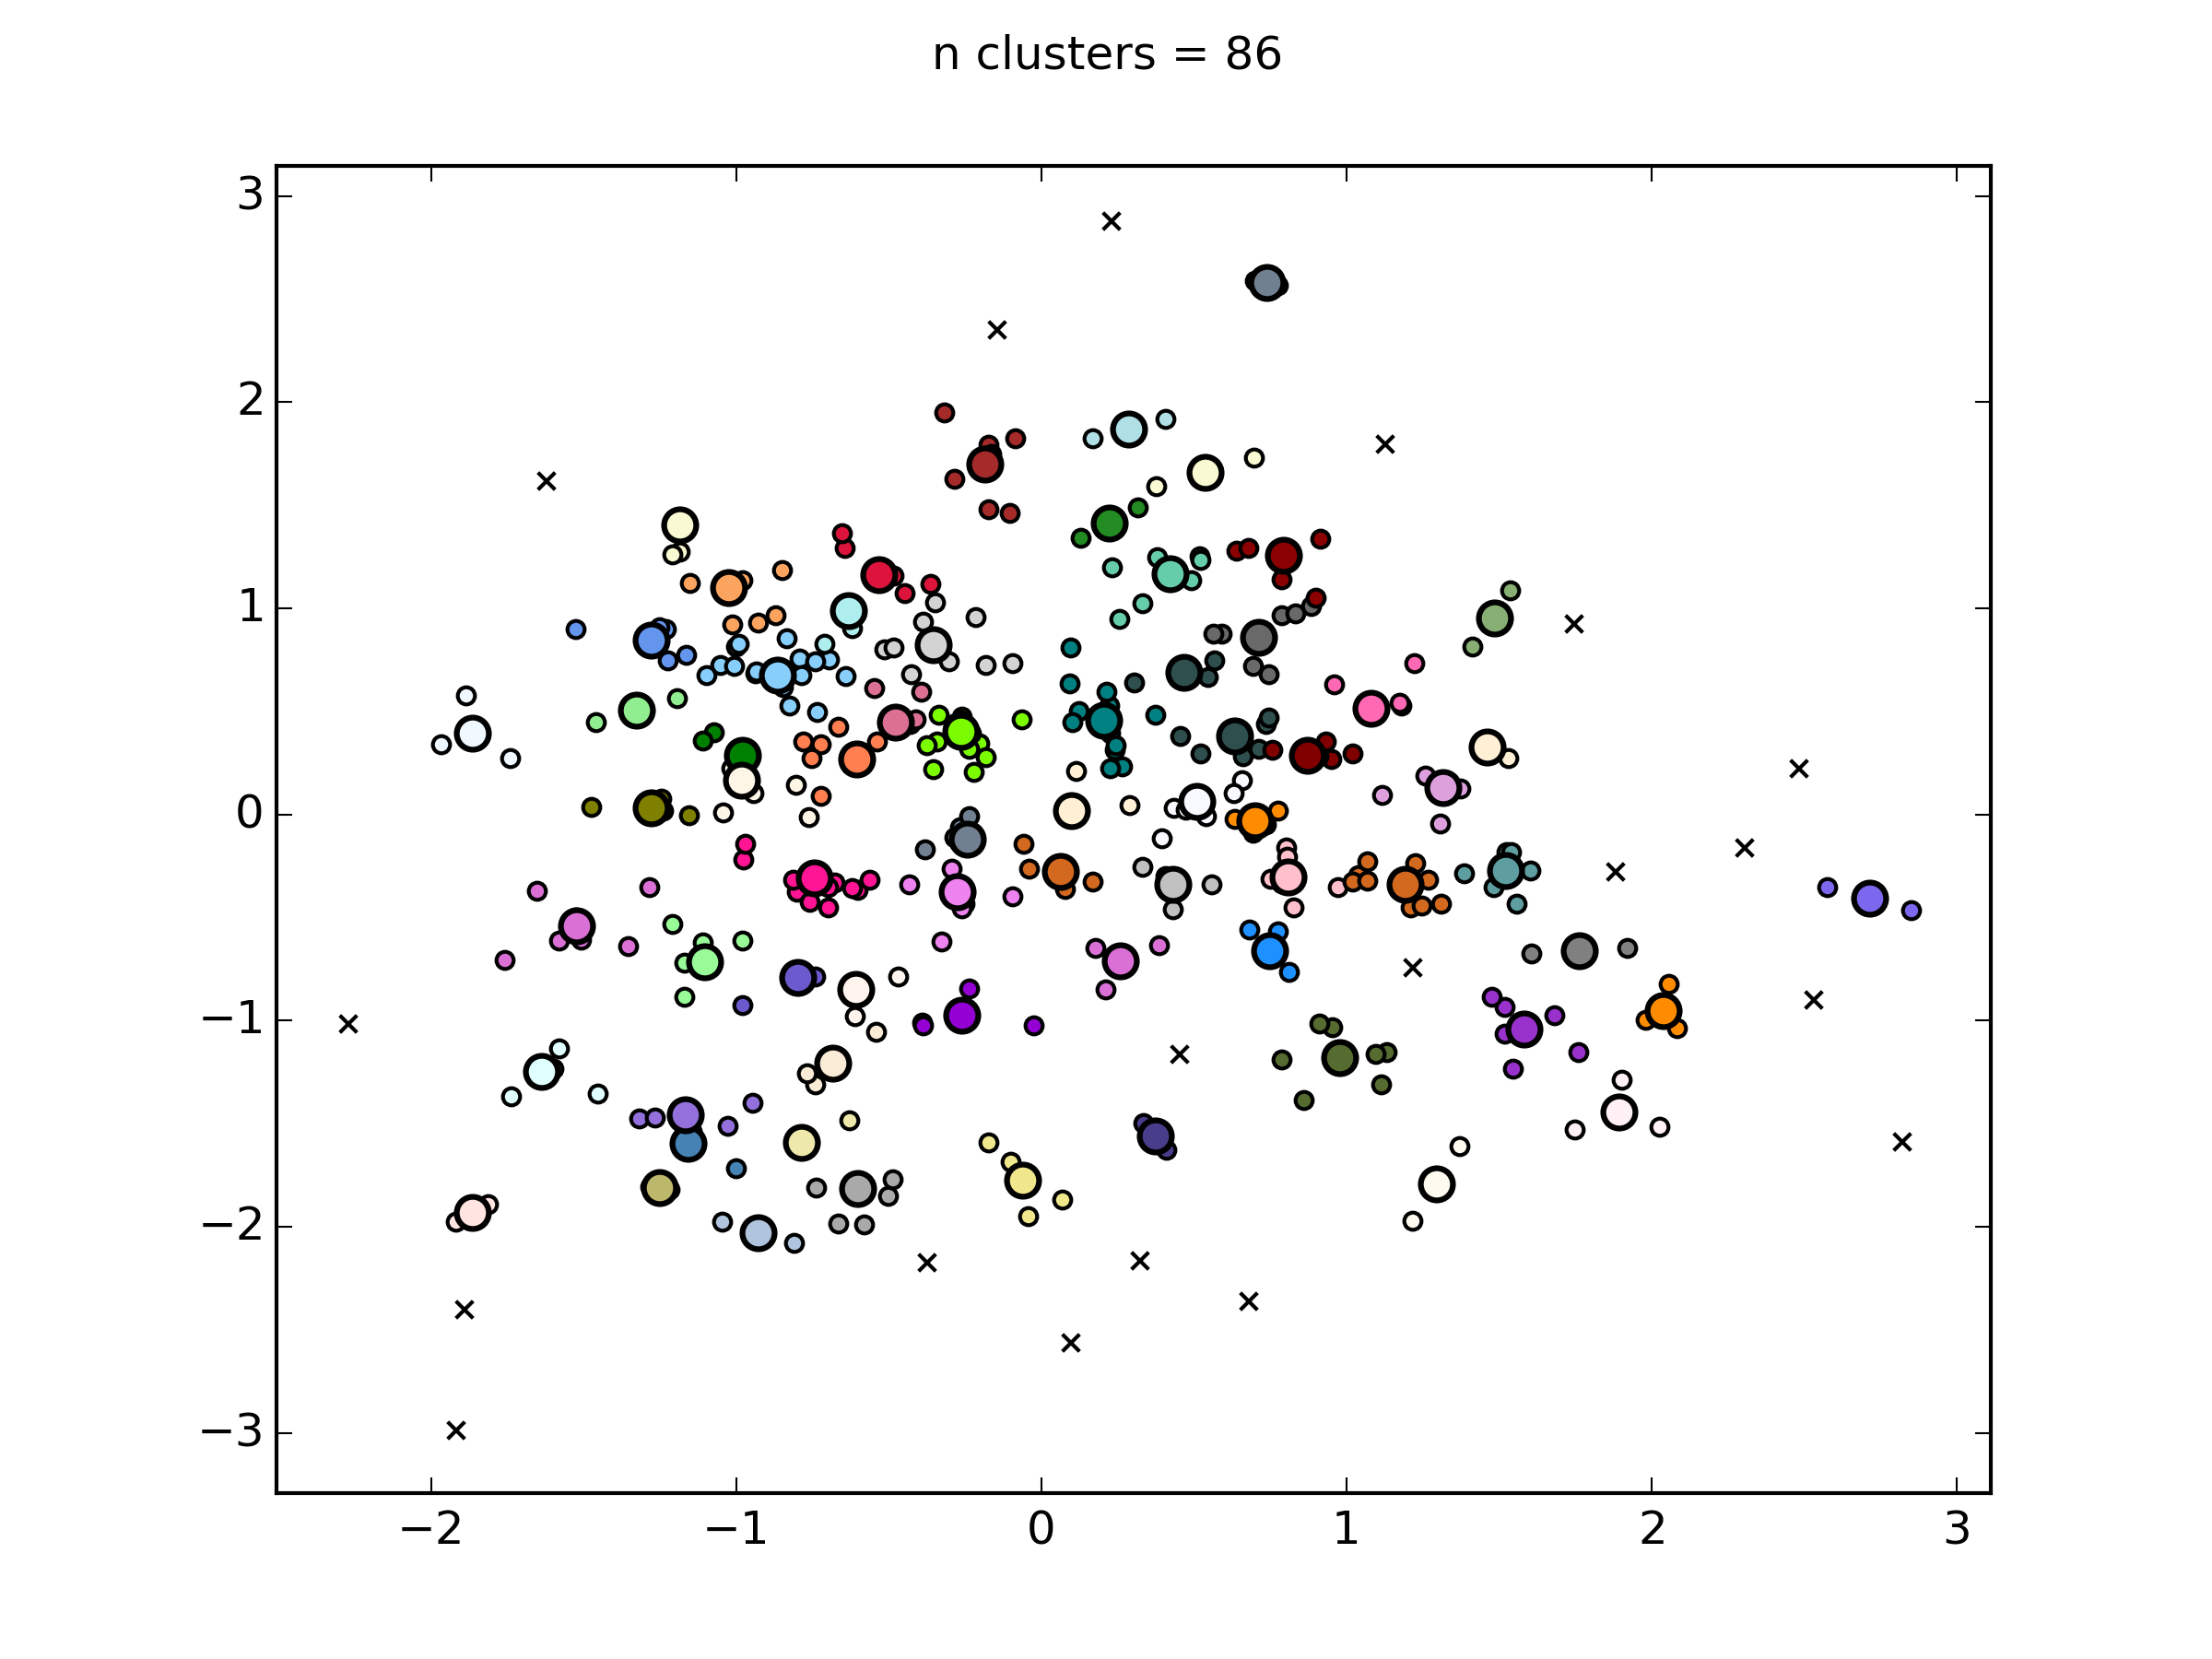
\includegraphics[width=0.9\textwidth]{birch_clustering.png}
      \caption{"BIRCH clustering of a single day"}
      \label{birch_clustering}
  \end{figure}

The data at hand does not stem from the BBC data set but from daily scraped newspapers. The papers shall not be named due to legal reasons. It is reasonable to believe that even less important events have multiple cluster points from different news sources. One can see that the resulting clusters are small and well formed. Some cluster centers are bigger than others. In those cases we can recluster them to further enhance the variance of clusters. The structures resemble that there are news that are covered several times a day and some that are not. Singleton clusters that are presented as x for one time events. Those outliers can be reclustered in a different run and would cover news like ``other''. The last figure \ref{mean_shift_clustering} is a clustering with the \emph{Mean Shift} algorithm. It is a partitonal algorithm working with density distributions, automatically inferring the size of clusters by a density threshold.

  \begin{figure}[h!]
    \centering
      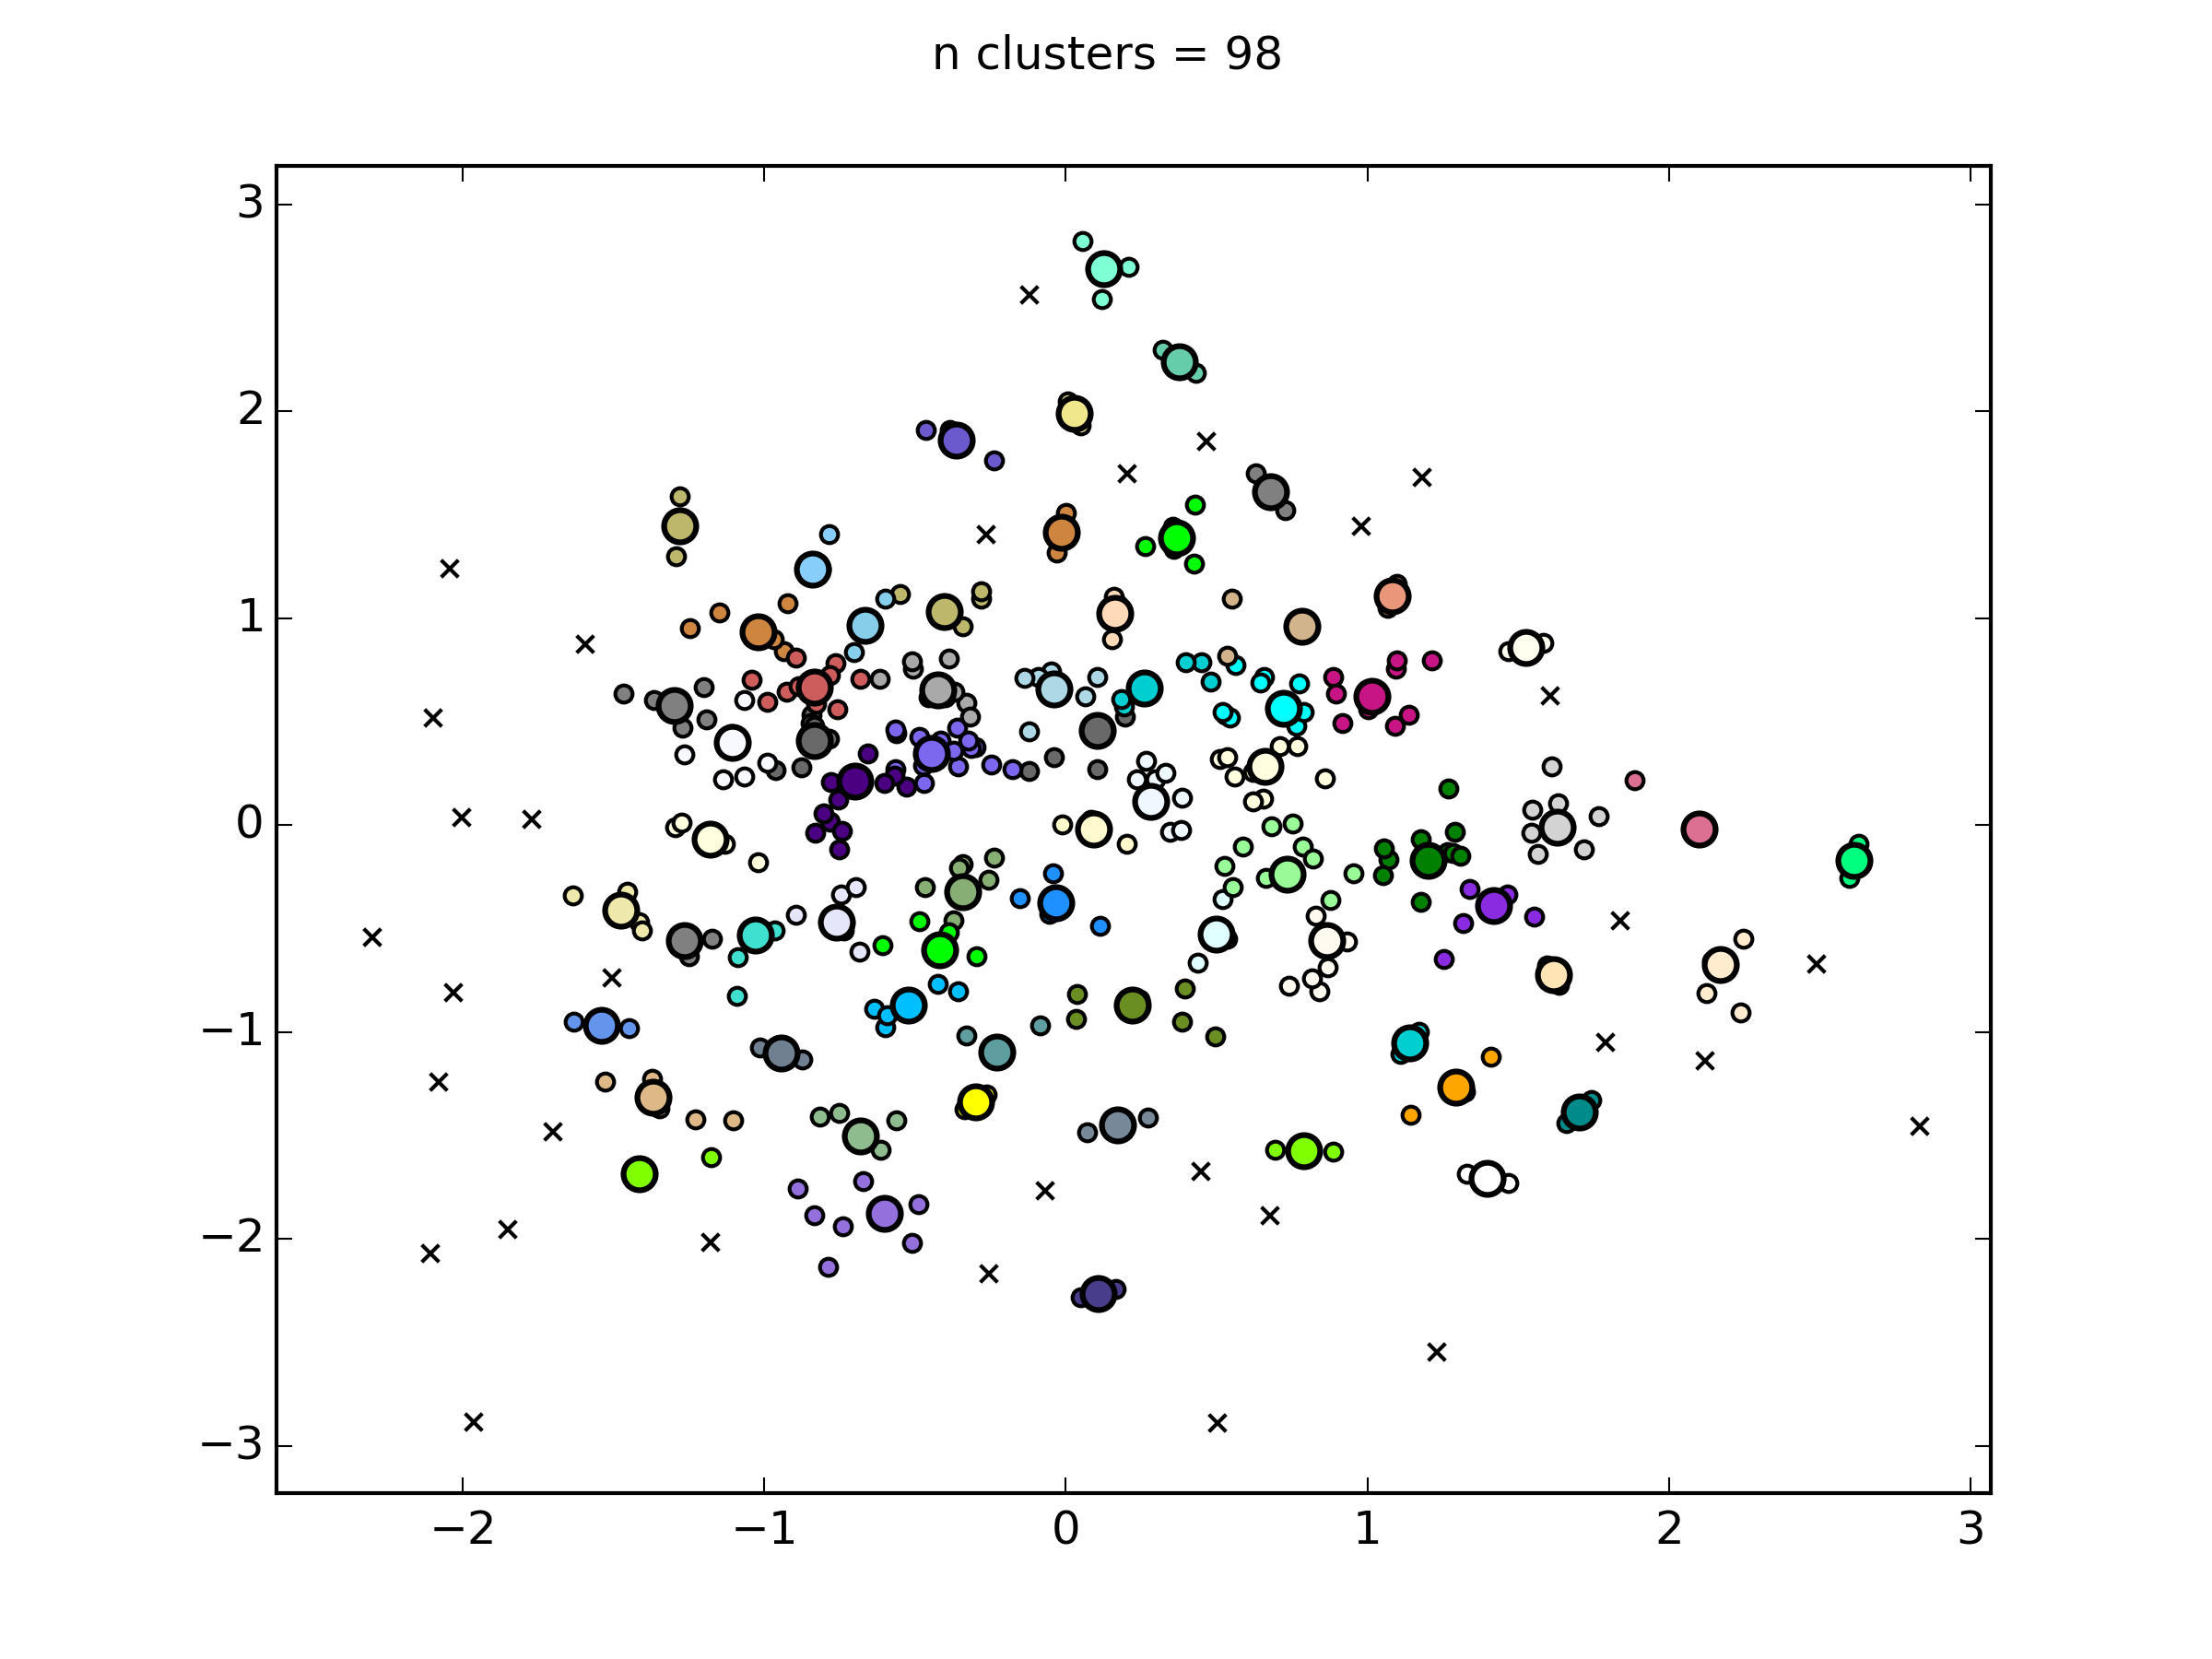
\includegraphics[width=0.9\textwidth]{mean_shift_clustering.png}
      \caption{"Mean Shift clustering of a single day"}
      \label{mean_shift_clustering}
  \end{figure} 

The clusters of the \emph{Mean Shift} are even smaller. The density threshold was carefully fine tuned over several runs. All visualizations were made of data containing roughly 350 documents from the category \emph{world} by two newspapers. Expecting at least 100 events covering different news. The final clusters visualizations are a result of several parameter estimations of the algorithms. All visualizations were done with the help of a Python API called \emph{matplotlib} by \cite{MatPlotHunter2007}.

\section{Multiple days clustering}
  Multiple days clustering was of the greatest interest while starting this thesis. It came to an understanding that it is inherently difficult to cluster and track documents over the course of several weeks. The time ran out to actually cluster multiple days in a row. Also, due to the problem of legality, the BBC data set came to the rescue. Multiple days clustering is an advancement on the single day clustering. See section \ref{sec:future_work} for future work.




      

    \chapter{Results and Discussion}
      \label{chapter:results_and_discussion}
      \epigraph{\emph{
  ``Simple models and a lot of data trump more elaborate models based on less data.''
}}{ Peter Norvig }

In this section the results of this thesis are discussed. The implementations are compared and evaluated. What is problematic and what worked out well? What can we conclude by now?

\section{Evaluation Analysis}
Comparing all implementations we can conclude, but.. etc.

\section{Pros and Cons}

\section{Conclusion}
  Some final words about measurement. It is highly debatable if any of the semantic enhancements has a measureable impact. If a user however views a website with summarizations of the daily news it makes a difference if phrases and references can be made to Wikipedia. It makes a difference in lexical diversity. Topic browsers with external knowledge sources are more diverse than browsers without. This cannot be measured in a mathematical way. The impact might be very small. The reason, the impact is so low is rather obvious: Without knowledge sources and Wordnet ontologies most clustering algorithms work just fine. Enhancing a good running model with additional feature selection heuristics can only make it better if there is mathematical proof that it does. It can certainly not proof if a human likes or dislikes the outcome.





    \chapter{Outlook}
      \label{chapter:outlook}
      \epigraph{\emph{
  ``All models are wrong, but some are useful.''
}}{ George E. P. Box }

\section{Summary}
\label{sec:summary}
Summing up all the pieces, this thesis provided a starting point of building a robust  news article summarization system. The groundwork on different clustering strategies were examined and several techniques of transformation from documents, to words, to coincidence matrices to statistical topical proportions were investigated. We heard a lot about feature selection and semantics, as well as different strategies on how to deal with word sense disambiguation. It was concluded that most of the strategies perform well but that the simplest of all models, namely by using the word tokens of a document, was superior to other approaches. Furthermore the data pipeline ``News-Clusty'' was evaluated and depicted. Several steps are necessary to get a vector of features from a real world document. Dealing with the noise and with the time drift effects by statistical techniques such as \lsa{} or \lda{} showed promising results. At last, we have shown how the clustering algorithm works on the BBC dataset and experimented, without giving any evidence, how the system works on real world data.

\section{Further Reading / Related Work}
\label{sec:further_reading}
In this section it is important to distinguish between the data pipeline and the quality of the algorithmic procedures. A generally well composed article about the different current approaches to clustering large and small documents is \cite{NextFrontierClustering2013}.\\

Several models of topic models were examined. There is more room to study the effects of \lda{} and certainly trying \hdp{}. For multi document summarization \lda{} can be used as a main approach, see \cite{MultiDocSumLDA2008}. The concepts of \hdpfull{} can be found in \cite{NonParametricBayes2007, HDP2006}. Further we could use Non-negative matrix factorization (NMF) as a matrix decomposition technique. See \cite{NMF1999} for a proper introduction.\\

While completely using unsupervised learning we could use artificial neural networks as well. A promising approach is the shallow neural network word2vec, that learns a feature representation using skip-gram models. See \cite{Word2Vec2014} for a good introduction.\\

Enhancing feature selection methods and more semantic relations promising work was done by \cite{NounPhraseSemanticClustering@2009@Zheng} using noun phrases for semantic clustering and 
\cite{WordNetAndFuzzyAssociation@2010@Chen} with \wordnet{} and soft assignment clustering. Further we can investigate external knowledge sources like \wiki{} to boost feature selection. Some good approaches were found in \cite{WikipediaClusteringSim2009} and \cite{WikipediaClustering2010}.\\

Time series clustering could not be tackled in this thesis. Beginning with basic introductions see \cite{ClusteringTimesSeriesSurves2005, RecentTechniquesClusteringSurvey2012, IncrementalClustering2012}. A good starting point for understanding topic models over time is \cite{BlogTopicLDA2013} analyzing blog posts.\\

The data pipeline is analogous to the Columbia Newsblaster System by \cite{NewsBlaster2002}. The whole literature evolving on the system is a vantage point for further reading. Also everything around the Google News aggregation system exemplified by \cite{GoogleNews2007}.\\

At last we have to mention the scalability issues. Working with algorithms across several server nodes needs different techniques. Algorithms need to be parallelized by techniques like map reduce, see \cite{MapReduce2008}. See parallel clustering approaches by \cite{ParallelClustering2009}.

\section{Future Work}
\label{sec:future_work}
Future work needs to be done on several things in the data pipeline.

\begin{description}
  \item[First] scaling and enhancement for data sets. This includes adding more newspaper data. In reality the classification system for news categories needs to be normalized across all newspapers. Finding ways of detecting the label of a document when downloading an article.
  \item[Second] adding a multi-document summarization system that works with the clustering.
  \item[Third] a routing system that detects the kind of event by biographical, single and multi events.
  \item[Fourth] scaling the clustering algorithms to several days by strategies mentioned in the experimental multiple days section.
  \item[Fifth] adding more feature selection strategies with \wordnet{}, \wiki{} and word2vec.
  \item[Sixth] using more advanced algorithms, especially topic modeling and semi supervised kernel methods.
  \item[Seventh] including external knowledge sources that work during the clustering methods as well.
  \item[Eighth] using state of the art distributed file systems to ease the task of feature selection and clustering
\end{description}

None of the above tasks is trivial. Each would greatly enhance the systems performance and usability. In theory the accuracy can be enhanced by incorporating more reliable and complex models to the clustering task. In total the system could be further prepared to run on international data sets from official conferences. A compact evaluation of the status quo against other systems was currently not possible. The status of the system is still in alpha stadium and thus, not production ready.

\subsection*{Multiple days clustering}
  The proposed model, seen in figure \ref{time_clustering}, is by clustering consecutive days without any overlap. After this, all cluster centers are consecutively merged and reassigned. The merging is based on similarity thresholds. If the similarity is high enough or we find hard evidence, like a named entity, cluster centers can be merged. Otherwise the clusters are kept separate. Going further we can set hard thresholds, how old a cluster should be, before it is not being considered anymore. Deciding when a merge, a reassignment or a new cluster emerges is the goal.

    \begin{figure}[h!]
      \centering
        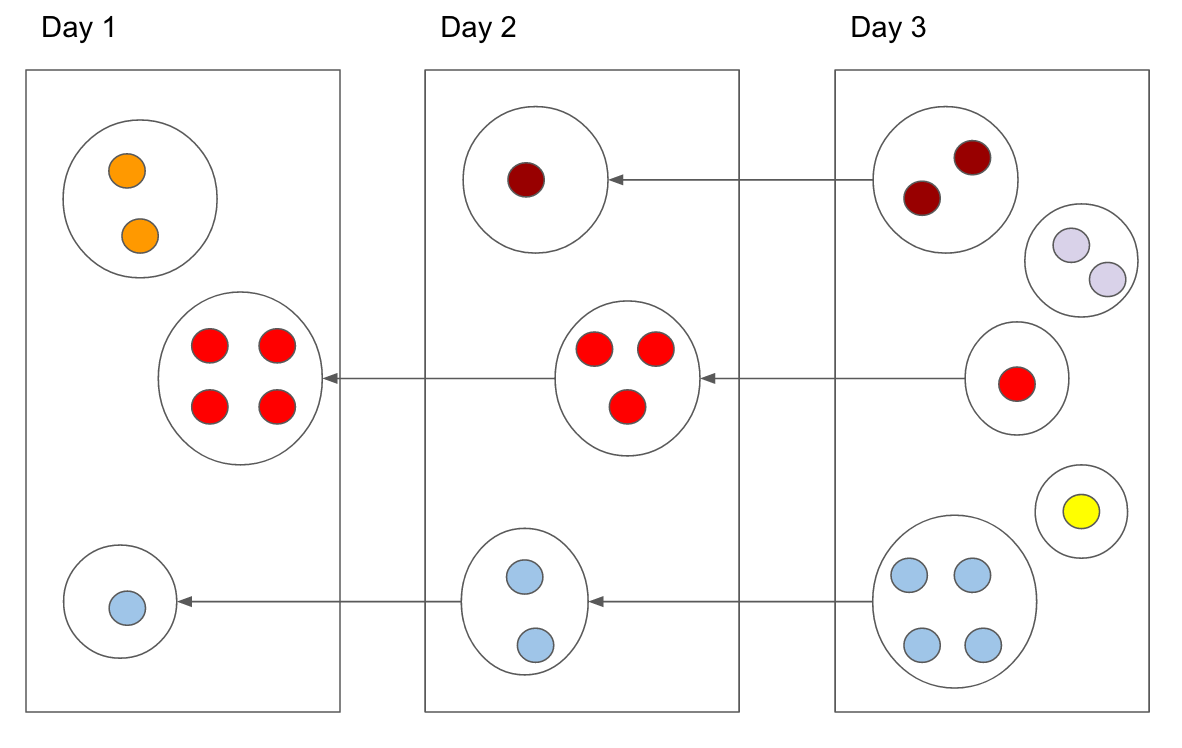
\includegraphics[width=0.7\textwidth]{time_clustering.png}
        \caption{"Multiple days clustering consecutive"}
        \label{time_clustering}
    \end{figure} 

  Several important enhancements to single day clustering must be made.

  \begin{description}
    \item[First] we need timestamps for each document
    \item[Second] we need to track documents over the course of several days. As the document size grows, algorithms need to be rethought for online or batch variations. In \cite{BlogTopicLDA2013} is a comprehensive analysis of blogs over time using \lda{}.
    \item[Third] solutions to over fitting must be found. That is, assigning too many documents to an existing cluster center.
    \item[Fourth] biasing must be avoided by inflating clusters that are of the same topics.
    \item[Fifth] measures have to be rethought. The silhouette coefficient will grow small with more documents in vector space. Different results are not comparable.
  \end{description}

  The content of this section is open for future work. Later we will discuss some articles dealing with the problem.

\section{Final Words}
We conclude this thesis with a quote of George E. P. Box, \emph{``All models are wrong, but some are useful.''}. I find this especially true for a domain, where text is seen as a system of linear combinations. In this sense, thank you very much for reading.


      

  \backmatter
    \typeout{===== Section: literature}
    \bibliographystyle{apalike}
    \bibliography{thesis}

    \addcontentsline{toc}{chapter}{Glossary}
    \renewcommand{\nomname}{Glossary}
    \markboth{\nomname}{\nomname}
    \printnomenclature
    \clearpage

    \typeout{===== Section: index}
    \printindex

    \HAWasurency

\end{document}
